\setchapterpreamble[u]{\margintoc}
\glsresetall % reset glossary
\chapter{Optimizing the layout of the modules in space} \label{chap:06}
Chapter~\ref{chap:05} introduced the foundational concepts of modular structures and formulated an optimization algorithm designed to optimize structures exhibiting the repetition of a single module topology. Additionally, it conducted a design of experiments to gain insights into the general mechanical behavior of modular structures. We observed that, especially in terms of volume, such structures are significantly penalized when compared to monolithic structures. Towards the end of the chapter, we identified two concepts that could potentially bridge this gap and enhance the performance of modular structures: the incorporation of multiple module topologies and the presence of empty subdomains in the structure where not structurally necessary. In this chapter we formulate an optimization algorithm that incorporates these two improvements.

The chapter is outlined as follows: In \secref{sec:06_opt}, we present an innovative optimization algorithm for modular structures, which concurrently optimizes both the layout and topology of the modules. The initial layout for the optimization is determined by identifying similarly behaving subdomains through a k-means clustering technique. \secref{sec:06_num_app} tests the proposed formulation on multiple two- and three-dimensional cases, considering both normalized and real engineering dimensions and material data.

\section{Optimize the modules' layout using a modified DMO algorithm} \label{sec:06_opt}
The objective of this chapter is to address the concurrent optimization of both the layout and topology of multiple modules within a modular structure. The key scientific challenge lies in the discrete nature of the layout optimization problem \ie find the optimal distribuition of the different modules within the subdomains of the structure, an inherently discrete problem. Given our intent to employ a gradient descent algorithm \sidecite{sigmund_usefulness_2011}, it is imperative to design a methodology for converting the discrete nature of the problem into a continuous one, permitting the application of gradient-based optimization techniques.

\subsection{Definition of the subdomains cross-sectional areas}
In this study, our strategy for addressing the discrete layout problem of modules as a continuous one involves defining the variables of the subdomains (i.e., the structure's variables) as a weighted sum of the module variables. This approach draws inspiration from the seminal work of Stegmann and Lund in the \gls{dmo} algorithm \sidecite{stegmann_discrete_2005}, where an optimizer selects from a set of fixed tensors the optimal homogenized stiffness tensor for each subdomain to minimize the compliance of a given structure. In the scenario of discretizing a ground structure into $N_\text{sub}$ subdomains and utilizing $N_\text{T}$ distinct modules, the cross-sectional areas of subdomain $j$ are expressed as:  
\begin{equation}
    \vect{a}^j = \sum_{t=1}^{N_\text{T}} w_t^j \bar{\vect{a}}_t 
\end{equation}
where $\bar{\vect{a}}_t $ represent the vector of cross-sectional areas of the $t$ module and $\vect{w}^j$ is the vector of weight relatives to the $j$ subdomain, defined as $ \vect{w}^j \in \mathbb{R}^t\,|\,w_j^t \in [0,1]$.

An example of a cantilever beam with $N_\text{sub}=8$ and $N_\text{T}=2$ is illustrated in \figref{fig:06_weighted_sum}, in which we visually show the impact of modifying the weight values $w$ on the structure topology.

\begin{figure*}
    \centering
    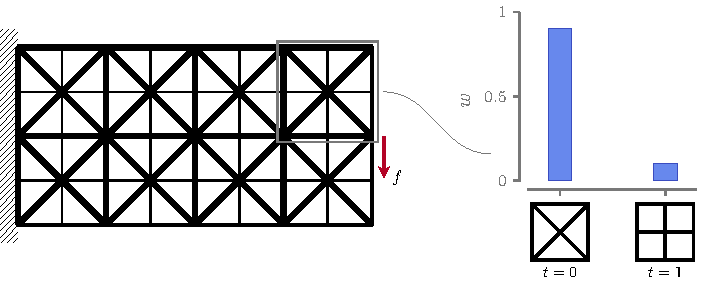
\includegraphics{figures/06_DMO/00_weight_dmo/weight_dmo.pdf}
    \caption{A modular cantilever beam with $N_\text{sub}=8$. The subdomains' topology is defined as the weighted sum of two modules' topologies.}
    \label{fig:06_weighted_sum}
\end{figure*}

\subsection{Variables penalization schemes}
The inherent limitation of the proposed approach is that, when the optimizer converges to a solution, the weights of all subdomains must converge to either zero or one, with the additional constraint that only one weight per subdomain can be equal to one. This condition is necessary to avoid intermediate weights, which would imply a combination of multiple modules' topologies lacking mechanical significance and proving impractical for manufacturing. To address this issue, we implement an interpolation scheme that penalizes intermediate weights. Specifically, we opt for the \gls{ramp} method \sidecite{stolpe_alternative_2001} instead of the more commonly used \gls{simp} interpolation scheme. This choice is motivated by \gls{ramp}'s advantageous property of ensuring that the derivative is never infinite nor zero when the weights approaches a value of zero.

We define the design variable $\matr{\alpha}\in\mathbb{R}^{j,t}$ as the modules' layout variable, responsible for the module selection within the subdomain $j$. Its relationship with the weight $w$ is the following:
\begin{equation}
    w_t^j = \frac{\alpha_t^j}{1+p(1-\alpha_t^j)}    
\end{equation}
where $p \in \mathbb{R}^+$ denotes a parameter governing the steepness of the \gls{ramp} interpolation. Drawing inspiration from the works of Hvejsel \etal \sidecite{hvejsel_material_2011}, we introduce a multi-phase variant of the \gls{ramp} interpolation, in which we concurrently penalize mechanical properties while artificially increasing the volume of modules with intermediate densities. To achieve this, we introduce an additional \gls{ramp} parameter, $q$, always negative ($q \in \mathbb{R}^-$), utilized to assess the augmented weights associated with the volume evaluation $V$. We can then write:
\begin{equation}
    V = \sum_{j=1}^{N_{\text{sub}}}\vect{\bar{\ell}}^T\tilde{\vect{a}}^j,
\end{equation}
where the vector $\tilde{\vect{a}}^j$, representing the increases cross-sectional areas of the $j$-th subdomain is defined as:
\begin{equation}
    \tilde{\vect{a}}^j = \sum_{t=1}^{N_\text{T}} \tilde{w}_t^j \bar{\vect{a}}_t, 
\end{equation}
and where $\tilde{w}$ is:
\begin{equation}
    \tilde{w}_t^j = \frac{\alpha_t^j}{1+q(1-\alpha_t^j)}.    
\end{equation}
So for every design variable $\alpha$, we associate two different weights $w$ and $\tilde{w}$ that are used to evaluate the mechanical properties and the structure volume, respectively (see \figref{fig:06_ramp}).


\begin{figure}
    \centering
    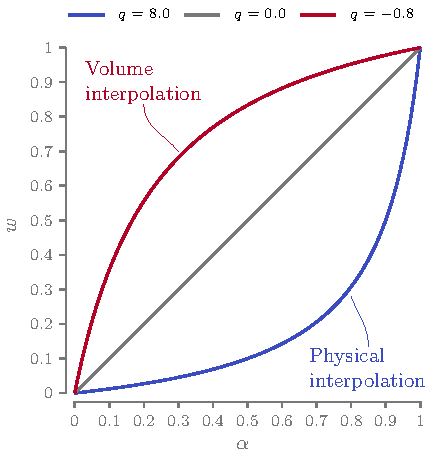
\includegraphics{figures/06_DMO/00_ramp/ramp.pdf}
    \caption{A dual-phase RAMP interpolation scheme is used to penalize the intermediate weights and promote 0-1 designs.}
    \label{fig:06_ramp}
\end{figure}

\subsection{The optimization formulation and resolution algorithm}
The objective function of the optimization process is the volume minimization of the modular structure. The members of the structure are subject to multiple mechanical constraints, namely stress, topological buckling, minimum slenderness, and compatibility constraints. Formulation $\mathbb{M}_1$ is stated in terms of modules' cross-sectional area $\bar{\vect{a}}$, module selection variables $\vect{\alpha}$, member forces $\vect{q}$, and nodal displacements $\vect{U}$ as follows:
\begin{equation}
    \begin{aligned}
    \min_{\bar{\vect{a}}, \vect{\alpha}, \bm{q}, \bm{U}}   && V &= \sum_{j=1}^{N_{\text{sub}}}\vect{\bar{\ell}}^T\tilde{\vect{a}}^j && \textrm{(Volume minimization)}\\
    \textrm{s.t.}   && \bm{B}\bm{q} &= \bm{f} && \textrm{(Force equilibrium)}\\
                    && \bm{q} &= \frac{\bm{a}\bm{E}}{\bm{\ell}}\bm{b}^T\bm{U} && \textrm{(Compatibility constraints)} \\
                    && \bm{q} &\geq -\frac{\bm{s}\bm{a}^2}{\bm{\ell^2}} && \textrm{(Euler buckling constraints)} \\
                    && -\sigma_C\bm{a} &\leq \bm{q} \leq \sigma_T\bm{a} && \textrm{(Stress constraints)} \\
                    && \bar{\vect{a}}_{t,r}&\geq \bar{a}_{t,r=1} && r \in \mathcal{C}_{l,r}(\bar{\vect{a}}_t),\, \forall t \\
                    && 0 &\leq \bar{\vect{a}} \leq \frac{4 \pi \bar{\vect{\ell}}^2}{\lambda_{\text{max}}} && \textrm{(Slenderness limit)} \\
                    && \sum_{t=1}^{N_\text{T}} \alpha_t^j &\leq 1, \; \forall j && \textrm{(One selected module max.)} \\
    \end{aligned}
    \tag{$\mathbb{M}_1$}
    \label{eq:06_optim_complete}
\end{equation}

This formulation builds on the classic \gls{dmo} approach, adding multiple mechanical constraints and while operating on a ground structure. Additionally, we are not only selecting the best module for every subdomain by changing the value of $\alpha$ as classic \gls{dmo} does, but we are also optimizing the modules' topology simultaneously. This simultaneous optimization presents a more challenging task. The advantages of this formulation lie in dealing with a discrete problem using continuous design variables and a gradient-based optimizer. However, it comes with the drawback of increasing the problem size, as we are adding numerous additional design variables $\alpha$ that scale with the number of subdomains and the number of modules \ie a vector of size $\vect{\alpha}^j \in \mathbb{R}^t$ is defined for every one of the $j$ subdomains.

The design variables $\alpha$ are constrained by a set of constraints that limit the maximum sum of $\alpha$ of a submodule $j$ to be less than or equal to one. It is crucial to note that we treat this constraint as a disequality constraint rather than an equality. This allows the optimizer to set all $\alpha$ to zero, permitting the removal of the subdomain from the structure. The constraint $\vect{g}_\text{sum}$ is expressed as follows:
\begin{equation}
    \vect{g}_\text{sum}:=\sum_{t=1}^{N_\text{T}} \alpha_t^j \leq 1, \; \forall j 
\end{equation}

Problem \eqrefnotext{eq:06_optim_complete} is tackled using a modified version of the proposed two-step solving algorithm. In this approach, we initially solve a relaxed problem denoted as $\mathbb{M}_2$, where kinematic compatibility constraints are omitted. This relaxed problem is inherently nonlinear due to the introduction of the $\alpha$ design variables. For this iteration, we have chosen to solve it in this form without linearizing the buckling constraints.

The relaxed formulation $\mathbb{M}_2$, expressed in terms of modules' cross-sectional area $\bar{\vect{a}}$, module selection variables $\vect{\alpha}$, and member forces $\vect{q}$, is the following:
\begin{equation}
    \begin{aligned}
    \min_{\bar{\vect{a}}, \vect{\alpha}, \bm{q}}   && V &= \sum_{j=1}^{N_{\text{sub}}}\vect{\bar{\ell}}^T\tilde{\vect{a}}^j && \textrm{(Volume minimization)}\\
    \textrm{s.t.}   && \bm{B}\bm{q} &= \bm{f} && \textrm{(Force equilibrium)}\\
                    && \bm{q} &\geq -\frac{\bm{s}\bm{a}^2}{\bm{\ell^2}} && \textrm{(Euler buckling constraints)} \\
                    && -\sigma_C\bm{a} &\leq \bm{q} \leq \sigma_T\bm{a} && \textrm{(Stress constraints)} \\
                    && 0 &\leq \bar{\vect{a}} \leq \frac{4 \pi \bar{\vect{\ell}}^2}{\lambda_{\text{max}}} && \textrm{(Slenderness limit)} \\
                    && \sum_{t=1}^{N_\text{T}} \alpha_t^j &\leq 1, \; \forall j && \textrm{(One selected module max.)} \\
    \end{aligned}
    \tag{$\mathbb{M}_2$}
    \label{eq:06_optim_relax}
\end{equation}
Problem $\mathbb{M}_2$ is solved using a non-linear gradient-based optimizer that iteratively exploits first and second-order derivatives to achieve convergence. The computation of the Jacobian and Hessian matrices for this problem is not trivial, and the details are elaborated in \appref{app:01}.

Once problem $\mathbb{M}_2$ is solved, we prepare for the second step, in which the structure's layout is fixed (we remove $\vect{\alpha}$ from the second optimization), and the kinematic compatibility constraints are reintroduced. We use the optimized module layout $\vect{\alpha}^*$ to establish the fixed module layout on the structure and evaluate the mapping matrix $H$ used in the variable linking approach of problem $\mathbb{M}_{1,\text{VL}}$. The indices of the mapping matrix $H$ are determined as follows:
\begin{equation}
    h_{j,t} =
    \begin{cases}
      1 & \text{if $\alpha^*_{j,t} = \max(\vect{\alpha}^*_{j})$ and $\alpha^*_{j,t}>0.01$} \\
      0 & \text{otherwise.} 
    \end{cases}
\end{equation}
Subsequently, the compatibility constraints are reintroduced, and a \gls{fea} is conducted to evaluate the displacements $\vect{U}$ used in the starting point of the following optimization step. To mitigate the risk of becoming trapped in local minima, the second step is solved on a reduced design space. The solution $\vect{\bar{a}}^*$ of the first optimization is used to simplifying the initial ground structure, thereby eliminating elements from the optimization that fall below the specified threshold value $a_{\text{thr}}$:
\begin{equation}
    \bar{a}_i<a_{\text{thr}} \; \forall i, \text{ with }a_{\text{thr}} = \chi \; \max(\bar{\vect{a}}^*),
    \label{eq:06_thr}
\end{equation}
with the parameter $\chi$ is the cross-sectional area threshold value.

Now, with all the components in place, we can set up the variable linking formulation ${\mathbb{M}}_{1,\text{VL}}$, as defined in Chapter~\ref{chap:05}. This formulation is employed to optimize modular structures with a fixed modules' layout and provide the final optimized design.
\marginnote{Formulation ${\mathbb{M}}_\text{1,VL}$, defined in Chapter~\ref{chap:05} permits to optimize modular structures with fixed module layout using the variable linking approach. It is stated in terms of modular cross-sectional areas $\bar{\vect{a}}$, member forces $\vect{q}$ and nodal displacements $\vect{U}$ as follows:
\begin{equation*}
    \begin{aligned}
    \min_{\bar{\vect{a}}, \vect{q}, \vect{U}}   && V &= \vect{\ell}^{T}\vect{a}\\
    \textrm{s.t.}  && \vect{a} &= \sum_{t=1}^{N_\text{T}} \vect{h}_t\otimes\bar{\vect{a}}_t \\ 
    && \matr{B}\vect{q} &= \vect{f} && \\
    && \vect{q} &= \frac{\vect{a}E}{\vect{\ell}}\vect{b}^T\vect{U} &&  \\
    && \vect{q} &\geq -\frac{s\vect{a}^2}{\vect{\ell}^{*2}} &&  \\
    && -\sigma_c\vect{a} &\leq \vect{q} \leq \sigma_t\vect{a} &&  \\
    && \bar{\vect{a}}_{t,r}&\geq \bar{a}_{t,r=1}\\
    && 0 &\leq \bar{\vect{a}} \leq \frac{4 \pi \bar{\vect{\ell}}^2}{\lambda_{\text{max}}}, \\
    \end{aligned}
\end{equation*}
}
\subsection{Optimization initialization: a clustering algorithm to identify similarly behaving subdomains}
Solving the first step of the proposed optimization formulation, we not only adjust the design variables responsible for the modules' layout ($\vect{\alpha}$) but also optimize the modules' topology $(\bar{\vect{a}}$). However, a significant challenge arises in this problem due to the strong interdependence between them \ie the topology of the module is optimized in function of the layout and \textit{vice versa}. It becomes particularly challenging for a gradient-based optimizer to determine the appropriate direction to follow \eg to reduce the value of the cross-sectional area of a member, the optimizer could play with $\vect{\alpha}, \bar{\vect{a}}$ or potentially both at the same time. This is especially true when starting from a completely uniform initial point (as observed in the work of \sidecite{bakker_simultaneous_2021}). To mitigate this challenge, we provide a slightly influenced starting point for the optimization process. We influence the module topology design variable at iteration zero $\vect{\alpha}_\text{init}$ as follows:
\begin{equation}
    \alpha_{t,\text{init}}^j =
    \begin{cases}
        \frac{1}{N_\text{T}} \cdot 1.1  & \text{if the $j$-th subdomain has the $t$-th module selected,}\\
        \frac{N_\text{T} - 1.1}{N_\text{T}(N_\text{T} - 1)} & \text{otherwise.} \\
    \end{cases}  
\end{equation}

\begin{figure*}
    \centering
    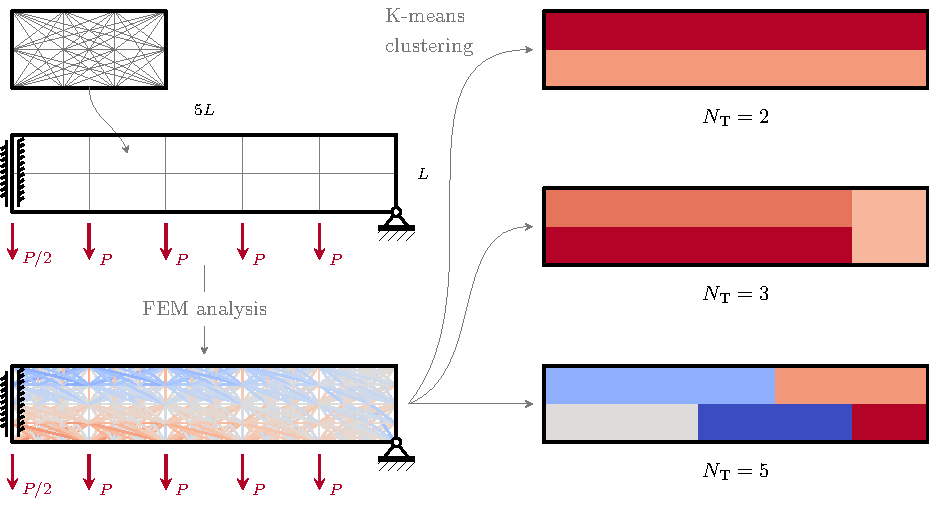
\includegraphics{figures/06_DMO/00_stress_clustering/stress_clustering.pdf}
    \caption{The stress values of the initial ground structure evaluated using a \gls{fem} analysis are used to identify similar behaving subdomains. The sets are calculated using the k-means clustering technique with $N_\text{T}$ number of clusters.}
    \label{fig:06_kmeans}
\end{figure*}

\begin{figure*}
    \centering
    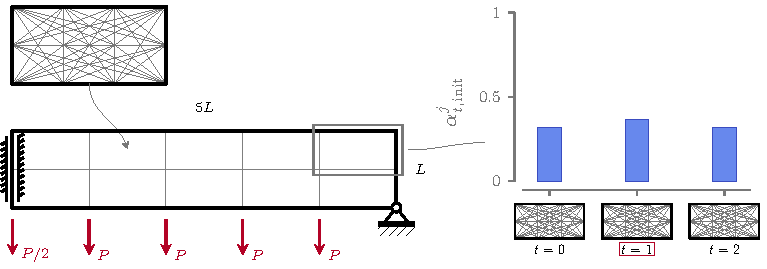
\includegraphics{figures/06_DMO/00_x0/x0.pdf}
    \caption{The proposed starting point for the first-step of the optimization: a fully-connected ground structure with uniform cross-sectional areas and a biased $\vect{\alpha}_\text{init}$ distribution, as suggested by the k-means clustering.}
    \label{fig:06_x0}
\end{figure*}

The idea behind how to select the best module for a subdomain is to identify subdomains that show similar mechanical behavior, grouping them based on their stress state. This grouping is assessed using a k-means clustering technique with the number of clusters equal to the number of module topologies $N_\text{T}$. Given a set of observations $(x_1, x_2, ..., x_{N_\text{sub}})$, where each observation is a $\bar{n}$-dimensional real vector, k-means clustering aims to partition the $N_\text{sub}$ observations into $N_\text{T}$ sets. In our context, each observation is the vector containing the \acrfull{fea} calculated stress distribution on the initial ground structure with a uniform cross-sectional area.

Additionally, besides the $\bar{n}$ stress values, we introduce the stress state $S$ for the $j$-th submodule as:
\begin{equation}
    S^j = \sum_{i=0}^{\bar{n}}|\sigma_i^j|
\end{equation}
This addition promotes the clustering not only of submodules loaded in similar ways but also based on similar magnitudes, thereby accounting for variations in voluminous and less voluminous modules.

The full clustering process is depicted in \figref{fig:06_kmeans}, showcasing how the grouping is conducted from the same starting point (FEA-calculated stress distribution on the uniform initial ground structure) but with different numbers of clusters ($N_\text{T}=2$, 3, and 5). Finally, \figref{fig:06_x0} illustrates the initial starting point of the optimization, with a uniform initialization of $\bar{a}$ and the biased weight distribution based on the k-means clustering.

\section{Numerical application}\label{sec:06_num_app}
The proposed algorithm to optimize layout and topology of modular structures is tested in this section against multiple two- and three-dimensional test cases. All examples presented are solved using a modified version of the proposed two-step formulation. In the first step, a relaxed formulation (without compatibility constraints) is solved to determine the optimized modules' layout and topology. Subsequently, the layout of the modules is fixed, and the optimization problem is solved again to ensure compliance with the compatibility constraints. Both formulations are solved using the nonlinear interior point solver IPOPT.

A continuation scheme is established on the penalization parameter $q$ of the \gls{ramp} interpolation scheme, utilized for evaluating the subdomains' volume. The parameter at the beginning of the optimization is set to zero and is then reduced to -0.4 and -0.8 each time the optimizer both satisfy the following criteria: the relative volume difference of two successive iterations $(V_i-V_{i-1})/V_i$ is less than $1 \times 10^{-4}$ and the optimizer is not in a restoration phase. This continuation scheme is implemented only on the $q$ parameter responsable for the volume evaluation. This because, as IPOPT is an interior point algorithm, and \marginnote{The cross-sectional area threshold value $\chi$ is used to threshold the bars of the original ground structure to reduce the number of candidates of the second step of the optimization. The candidates bars are the ones that satisfy the following inequality: $$\bar{a}_i<a_{\text{thr}} \; \forall i, \text{ with }a_{\text{thr}} = \chi \; \max(\bar{\vect{a}}^*)$$} increasing the $p$ parameter would place the optimizer well outside the feasible region each time it is increased, resulting in a suboptimal situation. The parameter $\chi$, referred to as the cross-sectional area threshold value, is set to $1 \times 10^{-4}$. 

The stopping criterion employed for the first step optimizations is $\|\Delta_{\text{NLP}}\|_\infty \leq \text{tol}_{nlp}$, where $\text{tol}_{nlp}=10^{-8}$. Here, $\Delta_{\text{NLP}}$ represents the scaled \gls{nlp} error, a comprehensive value used by IPOPT to consider both the optimality of the solution and constraint violations. The objective function is scaled such that the initial volume is 1000, the areas fall within the interval $[0,100]$, the initial forces range within $[0,100]$, and the $\alpha$ design variables lie within $[0,1]$. Several additional parameters are utilized in the first optimization step for CyIpopt and IPOPT:
\begin{itemize}
    \item \texttt{mu\_strategy} is set to \texttt{adaptive}
    \item \texttt{num\_linear\_variables} is set to \texttt{N}, where $N$ is the number of bars as the force is linear in this problem
    \item \texttt{grad\_f\_constant} is set to \texttt{yes}
    \item \texttt{bound\_push} is set to \texttt{1e-12}
    \item \texttt{constr\_viol\_tol} is set to \texttt{1e-6}
    \item \texttt{nlp\_scaling\_method} is set to \texttt{user-scaling}.
\end{itemize}
For the settings of the second step optimizer the reader can refer to Chapter~\ref{chap:05}.

\subsection{Layout optimization of fixed topology modules}
\begin{marginfigure}
    \centering
    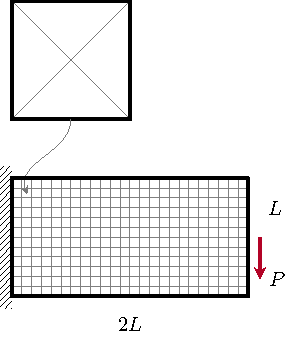
\includegraphics[width=\linewidth]{figures/06_DMO/00_cantilever_bcs/cant_mesh.pdf}
    \caption{Boundary conditions of the 2D cantilever beam divided in 24x12 subdomains. In the upper part of the image the ground structure of the module composed of $\bar{n}=6$ elements.}
    \label{fig:06_cant_BC_GS}
\end{marginfigure}
The proposed optimization formulation is highly versatile, allowing the solution of various optimization problems. We begin by optimizing the most straightforward modular structure problem. The objective is to optimize the distribution \ie the layout, of a single ($N_\text{T}=1$) fixed-topology module within a specified domain. The optimization process involves deciding whether each subdomain should be populated or not. For this scenario, we consider a single fixed module topology, setting $\bar{a}_i=0.6$ for all $i$. The only degree of freedom granted to the optimizer is, thus, the value of the weight $w$, controlled by the design variable $\alpha$.

The structure subject to optimization is a two-dimensional cantilever beam with dimensions $200\times100$, subjected to a center load of magnitude $P=1$ and directed downward. The optimization domain is divided into $24\times12$ subdomains along the X and Y axes, respectively. Each subdomain is populated with a simple fully connected $2\times2$ nodes ground structure comprising 6 candidate bars, as illustrated in \figref{fig:06_cant_BC_GS}. The units of the test case are normalized, and a list of the geometry and material parameters is provided in \tabref{tab:06_modular_cant_data}. In these examples, buckling and compatibility constraints are not taken into account for simplicity and to preserve the solution symmetry.

\begin{margintable}
    \small
    \centering
    \begin{tabular}{cc}
    \toprule
    \textbf{Parameter}        & \textbf{Value} \\ \midrule
    $L$              & 100     \\
    $\sigma_\text{c}, \sigma_\text{t}$ & $\pm 1$\\
    $P$              & 1   \\
    $a_\text{max}$              & 0.6   \\
    \bottomrule
    \end{tabular}
    \caption{Material data used for the 2D cantilever beam.}
    \label{tab:06_modular_cant_data}
\end{margintable}

Before showcasing and discussing the optimization results, we present two extreme cases that help us better understand and contextualize the optimization outcomes. First, we establish a monolithic optimization with no modular constraints, setting a maximum cross-sectional area $a_\text{max}=0.6$. The optimization is conducted on the same ground structure illustrated in \figref{fig:06_cant_BC_GS}. This result should represent a lower bound of the optimization, indicating the minimum value towards which modular optimization should tend; the closer to this value, the better. The resulting topology exhibits a volume $V=832.848$ and a structure resembling those obtained in classic topology optimization. Secondly, we present a fully modular structure, where all subdomains adopt the topology of the fixed topology module with all cross-sectional areas set to 0.6. In this case, the structure demonstrates a volume $V=9832.935$ and serves as the upper bound for the optimization. The topology of this fully modular structure is depicted in \figref{fig:06_cant_BC_cell}.

\begin{marginfigure}
    \centering
    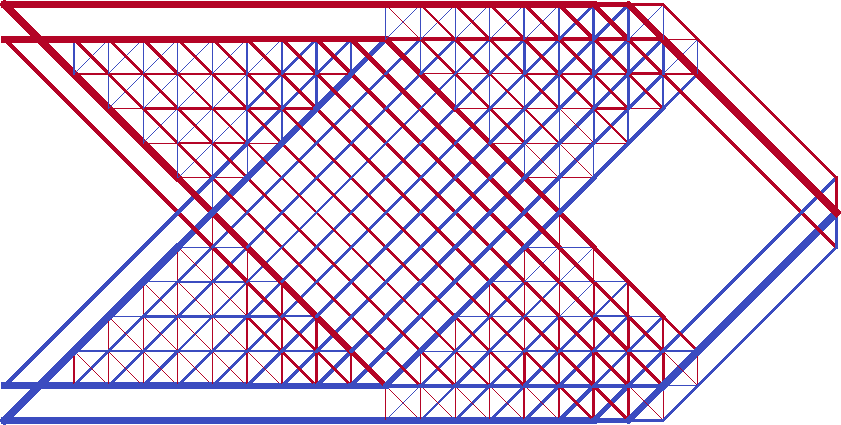
\includegraphics[width=\linewidth]{figures/06_DMO/00_cantilever_extremes/mono.pdf}
    \caption{Monolithic optimized structure for the cantilever beam 2D test case with a maximum cross-sectional area $a_\text{max}=0.6$. This solution represents the lower bound solution for this test case with a volume $V=832.848$.}
    \label{fig:06_cant_mono}
\end{marginfigure}


\begin{marginfigure}
    \centering
    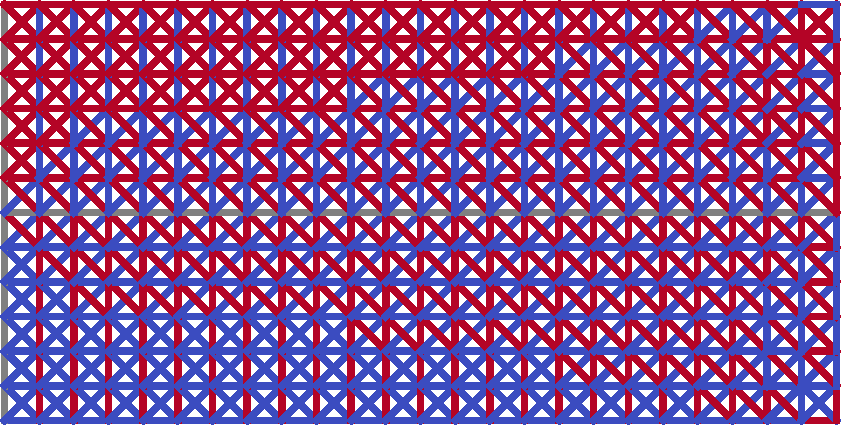
\includegraphics[width=\linewidth]{figures/06_DMO/00_cantilever_extremes/cell.pdf}
    \caption{Fully-modular structure in which every subdomain is populated with the given module. The structural volume is $V=9832.935$.}
    \label{fig:06_cant_BC_cell}
\end{marginfigure}

Now that we have established a reference for better understanding the optimization results, we proceed with the optimization of the layout of the fixed-topology module. For the first example, we decided not to penalize intermediate weights, setting $p=q=0$, and consequently $w=\alpha$. The optimized structure topology is illustrated in \figref{fig:06_fixed_module}a and \figref{fig:06_fixed_module}b, where we also depict the weight distribution of the solution. At this stage, the optimized structure exhibits a volume $V = 1567.216$, a value not significantly distant from the monolithic reference ($V=832.848$). However, this solution is non-physical as many subdomains display intermediate weights (see the weight distribution in \figref{fig:06_fixed_module}c), requiring a thresholding operation on the value of $\vect{w}$. The thresholding value is set to 0.01, such that any $j$ subdomain with a weight $w$ less than this value is considered empty. The result of the thresholding is presented in \figref{fig:06_fixed_module}d, where we observe that all weights are now set either to 1 or 0. The resulting structure has a volume $V = 8808.671$, indicating a noticeable volume increase due to the high number of intermediate weights in the solution shown in \figref{fig:06_fixed_module}b and very similar to the upper bound structure for the considered problem shown in \figref{fig:06_cant_BC_cell}.

\begin{figure*}
    \subcaptionbox{}{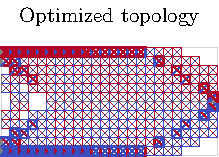
\includegraphics{figures/06_DMO/00_fixed_cells/top_00.pdf}}
    \hfill
    \subcaptionbox{$V = 1567.216$}{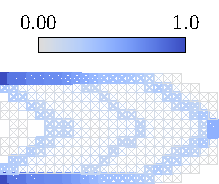
\includegraphics{figures/06_DMO/00_fixed_cells/weight_00.pdf}}
    \hfill
    \subcaptionbox{}{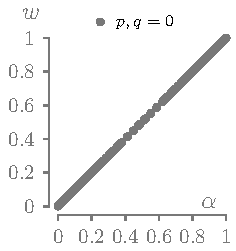
\includegraphics[height=3.5cm] {figures/06_DMO/00_fixed_cells/ramp_00.pdf}}
    \hfill
    \subcaptionbox{$V = 8808.671$}{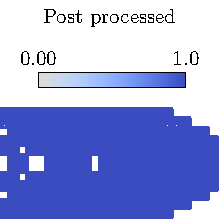
\includegraphics{figures/06_DMO/00_fixed_cells/weight_00_PP.pdf}}
    \bigskip
    \subcaptionbox{}{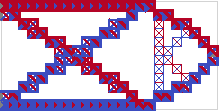
\includegraphics{figures/06_DMO/00_fixed_cells/top.pdf}}
    \hfill
    \subcaptionbox{$V = 1961.175$}{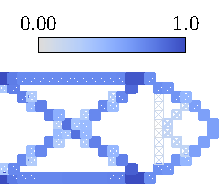
\includegraphics{figures/06_DMO/00_fixed_cells/weight.pdf}}
    \hfill
    \subcaptionbox{}{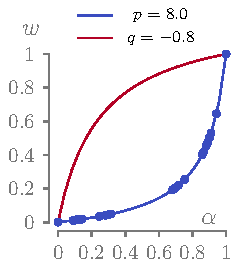
\includegraphics[height=3.5cm]{figures/06_DMO/00_fixed_cells/ramp.pdf}}
    \hfill
    \subcaptionbox{$V = 3414.214$}{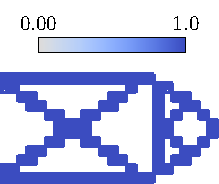
\includegraphics{figures/06_DMO/00_fixed_cells/weight_PP.pdf}}
    \caption{Optimization of the fixed module topology 2D cantilever beam. (a-d) shows the solution without penalizing intermediate weights with a final volume $V = 8808.671$; (e-h) shows the solution in which the RAMP interpolation helps reducing intermediate weights. The final structural volume is $V = 3414.214$.}
    \label{fig:06_fixed_module}
\end{figure*}

To address this issue, we implement a multi-phase \gls{ramp} interpolation where we simultaneously penalize mechanical properties (using the parameter $p$) and artificially increase the volume (using the parameter $q$) of modules with intermediate weights. In this optimization, we set $p=8$ and $q_{\text{min}}=-0.8$, and a continuation scheme is employed on the $q$ parameter to gradually decrease it to the minimum value, as explained in \secref{sec:06_num_app}. The optimized structure topology with penalized intermediate weights is depicted in \figref{fig:06_fixed_module}e and \figref{fig:06_fixed_module}f, with a resulting volume $V = 1961.175$, representing a \qty{25}{\%} increase compared to the unpenalized structure. However, it is evident that this solution presents fewer subdomains with intermediate weights, as reflected in the thresholding phase shown in \figref{fig:06_fixed_module}h, where the volume is now $V=3414.214$, more than \qty{60}{\%} less than the unpenalized structure. These behaviours are similar to what we already experienced with classic topology optimization \sidecite{bendsoe_material_1999,sigmund_non-optimality_2016}.

Now that we have assessed the need for a penalization scheme, we test the proposed optimization formulation with some test cases using multiple fixed modules. As the topology of the module ($\bar{a}$) is not modified, no perturbation is made to the initial starting point, and $\vect{\alpha}_\text{init}$ at iteration 0 is set to $\alpha_{t,\text{init}}^j = 0.5, \forall j, t$. 

The first test we conducted was to optimize the layout of two different modules ($N_\text{T}=2$) that present the same module topology connectivity but different cross-sectional areas. We used two 2-nodes fully connected modules with uniform cross-sectional areas set to 0.6 and 0.2 to simulate high and low density modules for high and low-stress parts of the structure. The results are presented in \figref{fig:06_multiple_fixed}a and b, and the optimized structure has a volume $V = 2987.437$. This represents a \qty{12}{\%} improvement over the single fixed topology.

\begin{figure*}
    \hspace*{\fill}
    \subcaptionbox{}{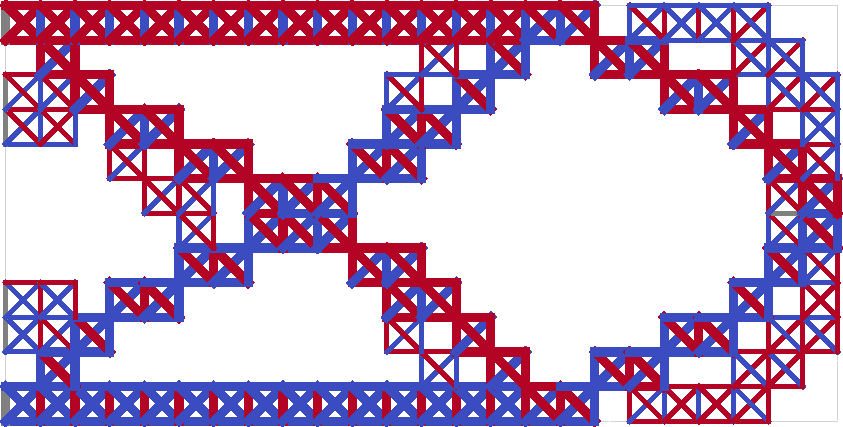
\includegraphics[height=2.5cm]{figures/06_DMO/00_fixed_cells_multiple/fig1-Topology_area.pdf}}
    \hfill
    \subcaptionbox{$V = 2987.437$}{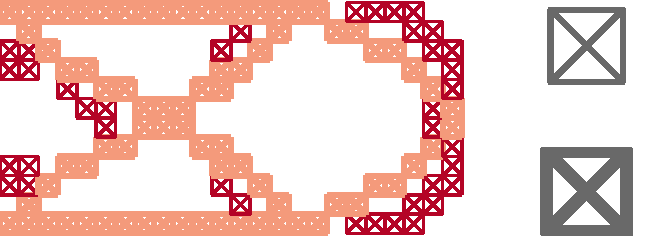
\includegraphics[height=2.5cm]{figures/06_DMO/00_fixed_cells_multiple/mod_area.pdf}}
    \hspace*{\fill}

    \bigskip

    \hspace*{\fill}
    \subcaptionbox{}{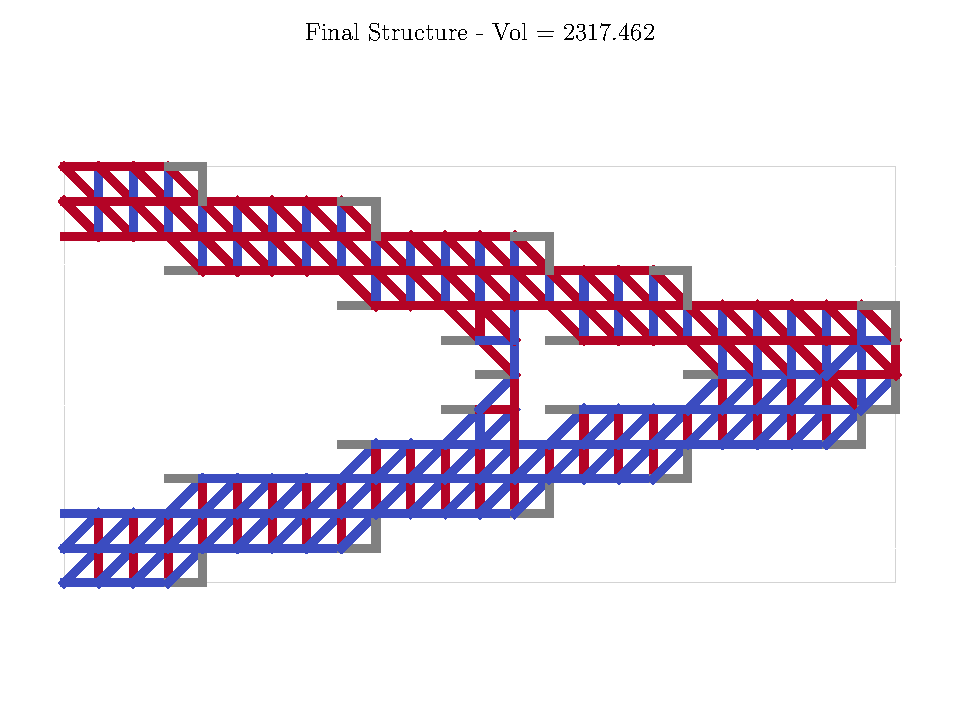
\includegraphics[height=2.5cm]{figures/06_DMO/00_fixed_cells_multiple/fig1-Topology_topol.pdf}}
    \hfill
    \subcaptionbox{$V = 2317.462$}{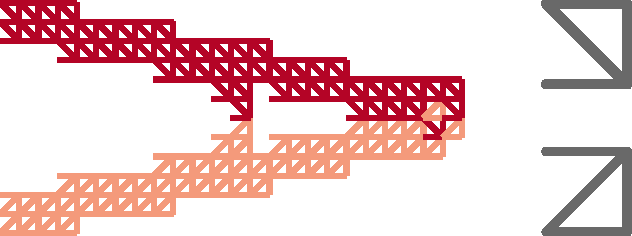
\includegraphics[height=2.5cm]{figures/06_DMO/00_fixed_cells_multiple/mod_topol.pdf}}
    \hspace*{\fill}
    \caption{Two different examples of the optimization of a modular 2D cantilever beam using $N_\text{T}=2$ fixed topology modules. (a-b) show the topology and the module layout of the structure obtained using two modules with identical topology, but different cross-sectional areas, while the solution showed in (c-d) is obtained using two modules with identical cross-sectional areas, but different topology. In (a) and (c) red bars are loaded in tension, while blue bars are loaded in compression.}
    \label{fig:06_multiple_fixed}
\end{figure*}

Similar results are presented in \figref{fig:06_multiple_fixed}c and d, in which we optimize the module layout of two modules that present different mirrored topologies (see \figref{fig:06_multiple_fixed}d). The structure optimized in this way exhibits a very different module layout and a final volume $V = 2317.462$, even better than before. These two examples confirm that giving more design freedom to the optimizer can enhance the mechanical performance of the modular structure.

\subsection{Modules and layout optimization}
We now optimize a modular structure using multiple modules that can vary their topology (the values of $\bar{a}$ are no longer fixed). In the case of $N_\text{T}=1$, the starting point for the value of $\vect{\alpha}_\text{init}$ is still trivial to evluate ($\alpha^j_\text{init}=1, \, \forall j$), and the resulting structure, along with the optimized module topology, is shown in \figref{fig:06_module_topol_opt}a and b. The modular structure exhibits a volume $V = 2107.983$, the best found until this point, confirming the interest in optimizing both the modules' topology and layout.

\begin{figure}
    \hspace*{\fill}
    \subcaptionbox{$V = 2107.983$}{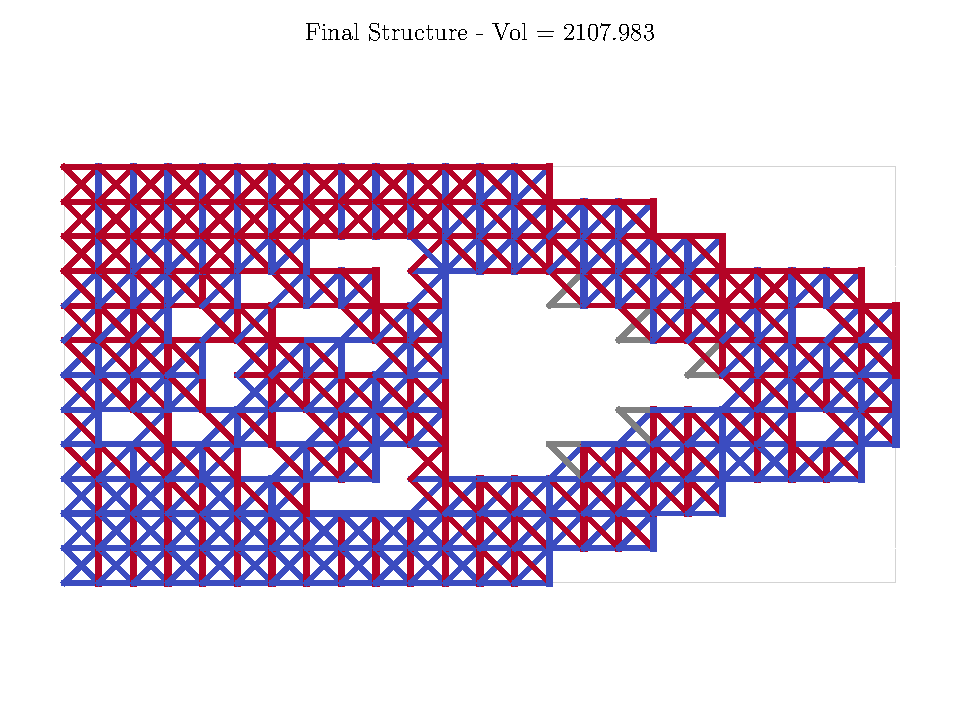
\includegraphics[height=2.5cm]{figures/06_DMO/00_optimized_module/fig1-Topology.pdf}}
    \hfill
    \subcaptionbox{}{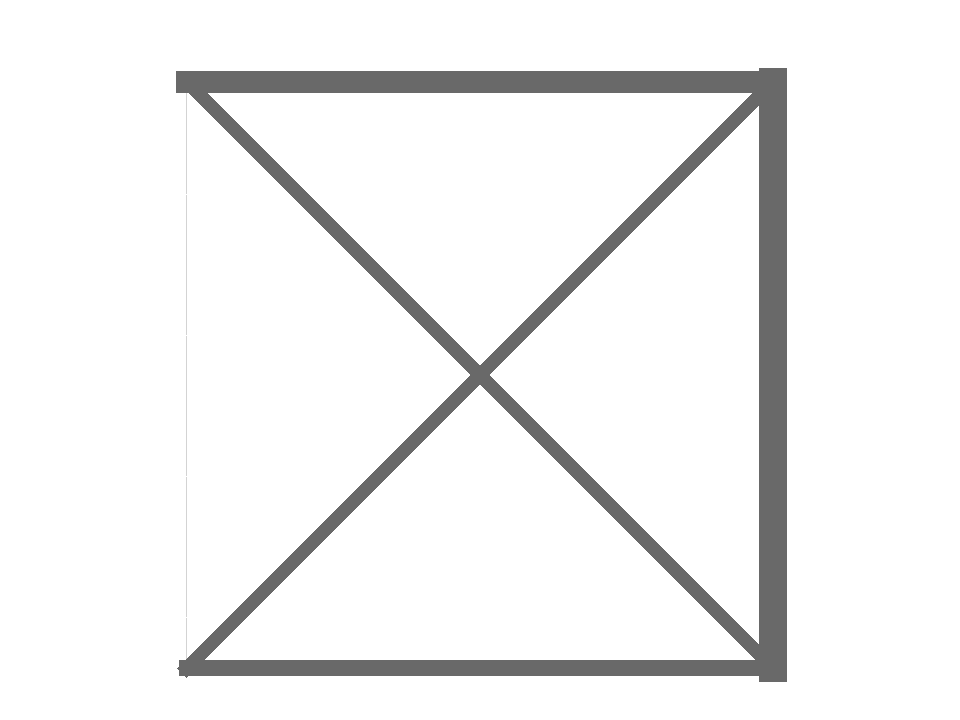
\includegraphics[width=0.3\linewidth]{figures/06_DMO/00_optimized_module/fig8-Module_Topology_001.pdf}}
    \hspace*{\fill}
    \caption{Optimized topology of the modular structure (a) and the module (b) for the 2D cantilever beam optimized using a single module ($N_\text{T}=1$). Red bars are loaded in tension, while blue bars are loaded in compression.}
    \label{fig:06_module_topol_opt}
\end{figure}

\begin{figure}
    \centering
    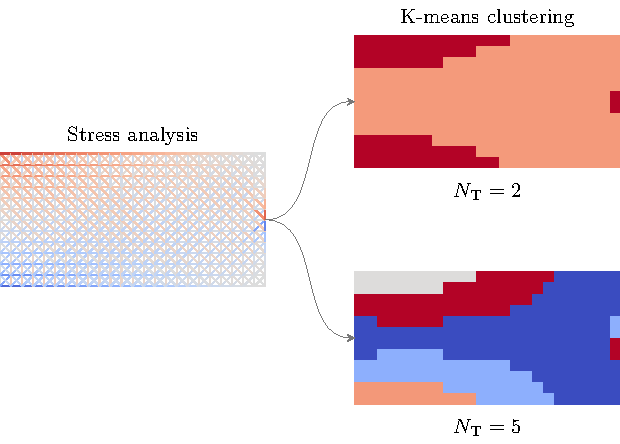
\includegraphics{figures/06_DMO/00_optimized_modules/kmeans.pdf}
    \caption{Similarly stressed submodules are identified using the k-means clustering algorithm to suggest a starting point for the first step of the proposed optimization algorithm. In the figure we show the resulting distribution for $N_\text{T}=2$ and $N_\text{T}=5$ obtained from the \gls{fea} stress.}
    \label{fig:06_cant_kmeans}
\end{figure}

Moving on to the layout and topology optimization of modular structures with a number of module topologies $N_\text{T} > 1$, it becomes necessary to employ k-means clustering to determine the initial values for the layout module variable  $\vect{\alpha}_\text{init}$. A \gls{fem} analysis is conducted on the starting ground structure with uniform cross-sectional areas, and the k-means clustering is used on the stress distribution using $N_\text{T}$ different clusters. This process is showed for $N_\text{T}=2$ and $N_\text{T}=5$ in \figref{fig:06_cant_kmeans}, where it is observed that, in general, the clusters tend to align with more and less stressed zones more than different type of stress solicitation \ie direction of principal stress, more compressive or tensile loads. This fact is particularly evident in the $N_\text{T}=2$ example. It is only when the number of clusters reaches $N_\text{T}=5$ that a distinction between tension and compression becomes apparent, resulting in a solution that is no more symmetrical with respect to the neutral axis of the beam.

\begin{table}
    \centering
    \small
    \begin{tabular}{lx{1.5cm}x{1.5cm}x{1.5cm}x{1.5cm}x{1.5cm}}
        \toprule
    $N_\text{T}$ & 1&2&3&4&5 \\ \midrule 
    $N_\text{sub}$& 288&288&288&288&288 \\
    $N_\text{sub, e}$ & 107&   45  &   72   &   43   &   50     \\
    $V$  & 2107.983 &  1722.606 &   1730.047  & 1589.899  & 1416.048  \\
    $a_\text{max}$      & 0.37& 0.35  & 0.48  &  0.54  & 0.53   \\
    $\varphi$   &\qty{17.16}{\percent}&\qty{17.86}{\percent}&\qty{14.20}{\percent}&\qty{17.95}{\percent}&\qty{16.65}{\percent}   \\
    $\psi$& 0.52   &  0.59 &  0.57   & 0.61  &0.67      \\
    t        & \hms{0;0;35}  &  \hms{0;0;18} & \hms{0;0;14} & \hms{0;0;17} & \hms{0;0;26}  \\ \bottomrule
    \end{tabular}
    \caption{Numeric results of the parametric study on the influence of the number of modules on the optimized 2D cantilever beam.}
    \label{tab:06_different_topol_cant}
\end{table}
\begin{marginfigure}
        \centering
        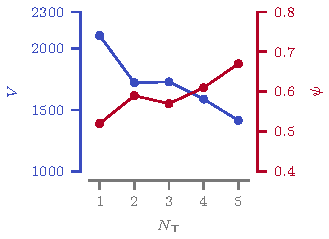
\includegraphics[width=\linewidth]{figures/06_DMO/00_multiple_modules_curves/multi_tab.pdf}
        \caption{Influence of the number of modules $N_\text{T}$ on the volume $V$ and the loading metric $\psi$ of the optimized 2D cantilever beam.}
        \label{fig:06_different_topol_cant_crv}
\end{marginfigure}

Starting from the advised starting point from the k-means clustering, the optimizations are performed for $N_\text{T}$ from 2 to 5, and their results are summarized in \tabref{tab:06_different_topol_cant}. Here are the main takeaways: looking at the evolution of the volume of the optimized structures with the different numbers of modules $N_\text{T}$, we notice how they behave as expected, as a monotonically decreasing function. This behavior could be explained by the general specialization of the modules that can shape their topology for more specific load cases and be less general-purpose, increasing the structure efficiency and reducing the redundancies. Indeed, we can observe that the value of the average bar load $\varphi$ is increasing with the number of module topologies. these two effects are illustrated in \figref{fig:06_different_topol_cant_crv}. Additionally, it is interesting how, with an increase in the number of module topologies, the number of empty subdomains $N_\text{sub, e}$ drops from 107 and stabilizes at around 50. This suggests that for this specific test case, employing more module topologies results in fewer empty subdomains, indicating that it is better to have many light modules rather than few strong and heavy ones. Concerning the calculation time, we observe no real correlation with the number of modules. We speculate that even if the number of design variables increases with the number of modules $N_\text{T}$, the problem is often easier to solve, and fewer iterations are necessary to attain convergence. The topology of the modular structure with $N_\text{T}=2$ and $N_\text{T}=5$ is shown together with their optimized modules in \figref{fig:06_diferent_modules_cant_topology}. Finally, it is interesting to notice how the optimized structures exhibit similar module layouts concerning the number of module topologies.


\begin{figure*}
    \subcaptionbox{$V=1722.606$}{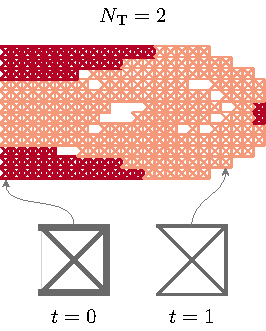
\includegraphics[width=0.3\linewidth]{figures/06_DMO/00_optimized_modules/nt2.pdf}}
    \hfill
    \subcaptionbox{$V=1416.048$}{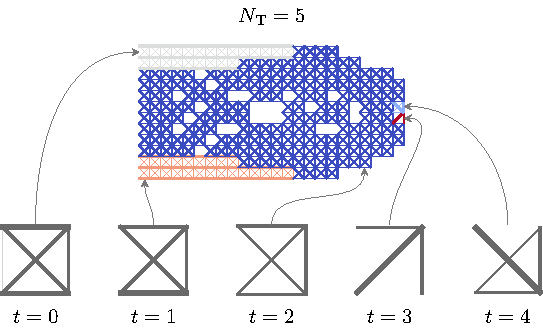
\includegraphics[width=0.6\linewidth]{figures/06_DMO/00_optimized_modules/nt5.pdf}}
    \caption{Visual representation of the optimized modular 2D cantilever beam together with the corresponding module topologies for (a) $N_\text{T}=2$  and (b) $N_\text{T}=5$.}
    \label{fig:06_diferent_modules_cant_topology}
\end{figure*}

\begin{marginfigure}
    \centering
    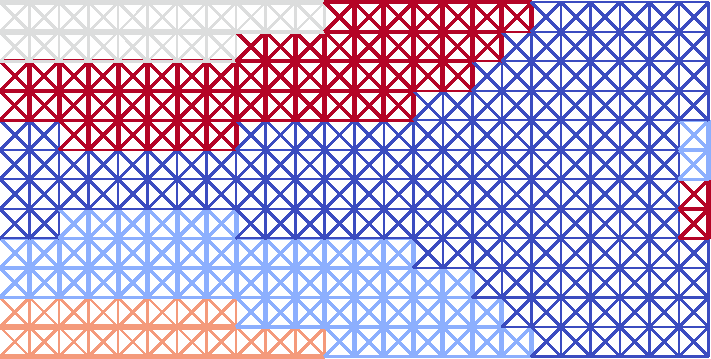
\includegraphics[width=\linewidth]{figures/06_DMO/00_optimized_modules/VL/nt=5VL.pdf}
    \caption{Optimized 2D cantilever beam obtained using the variable linking formulation with fixed modules' layout and $N_\text{T}=5$. The modules' layout is obtained using the k-means clustering technique. The final volume is $V = 1727.314$.}
    \label{fig:06_cant_variable_link}
\end{marginfigure}

The last aspect we want to comment on is a comparison between the optimized structure with $N_\text{T}=5$ presented in \figref{fig:06_diferent_modules_cant_topology}b and the structure we would obtain if we used the clustering algorithm-suggested module layout to set the mapping matrix $H$ and the variable linking algorithm described in \secref{sec:05_opt_formulation}. Using this formulation, the structure's layout is fixed, and no changes or empty modules are possible. The optimized structure using this algorithm is shown in \figref{fig:06_cant_variable_link}, and it has a volume $V = 1727.314$, more than \qty{20}{\percent} greater compared to the proposed method solution. The difference can be explained by two factors: firstly, the proposed formulation allows for empty subdomains, which significantly aids in lightening the structure. Secondly, the proposed formulation uses the clustering results only as a starting point for the layout of the optimization, but the layout can then evolve to a more optimized design. This example verifies the need to consider the module layout as a variable of the optimization that should be optimized simultaneously with the modules' topology.

\subsection{A benchmark case study: a simply supported modular bridge}
The proposed formulation and solution algorithm are now benchmarked against findings in the literature. To the knowledge of the authors, to this date there are no other works that optimize the layout and topology of modular structures using a gradient descent algorithm with continuous design variables. However, similar results have been achieved using \gls{mip}, \gls{milp} algorithms, or \gls{sa} to optimize modular structures. Examples include the works of Tugilimana \sidecite{tugilimana_spatial_2017, tugilimana_integrated_2019}, and we will now compare the results of the proposed formulation with them.

\begin{marginfigure}
    \centering
    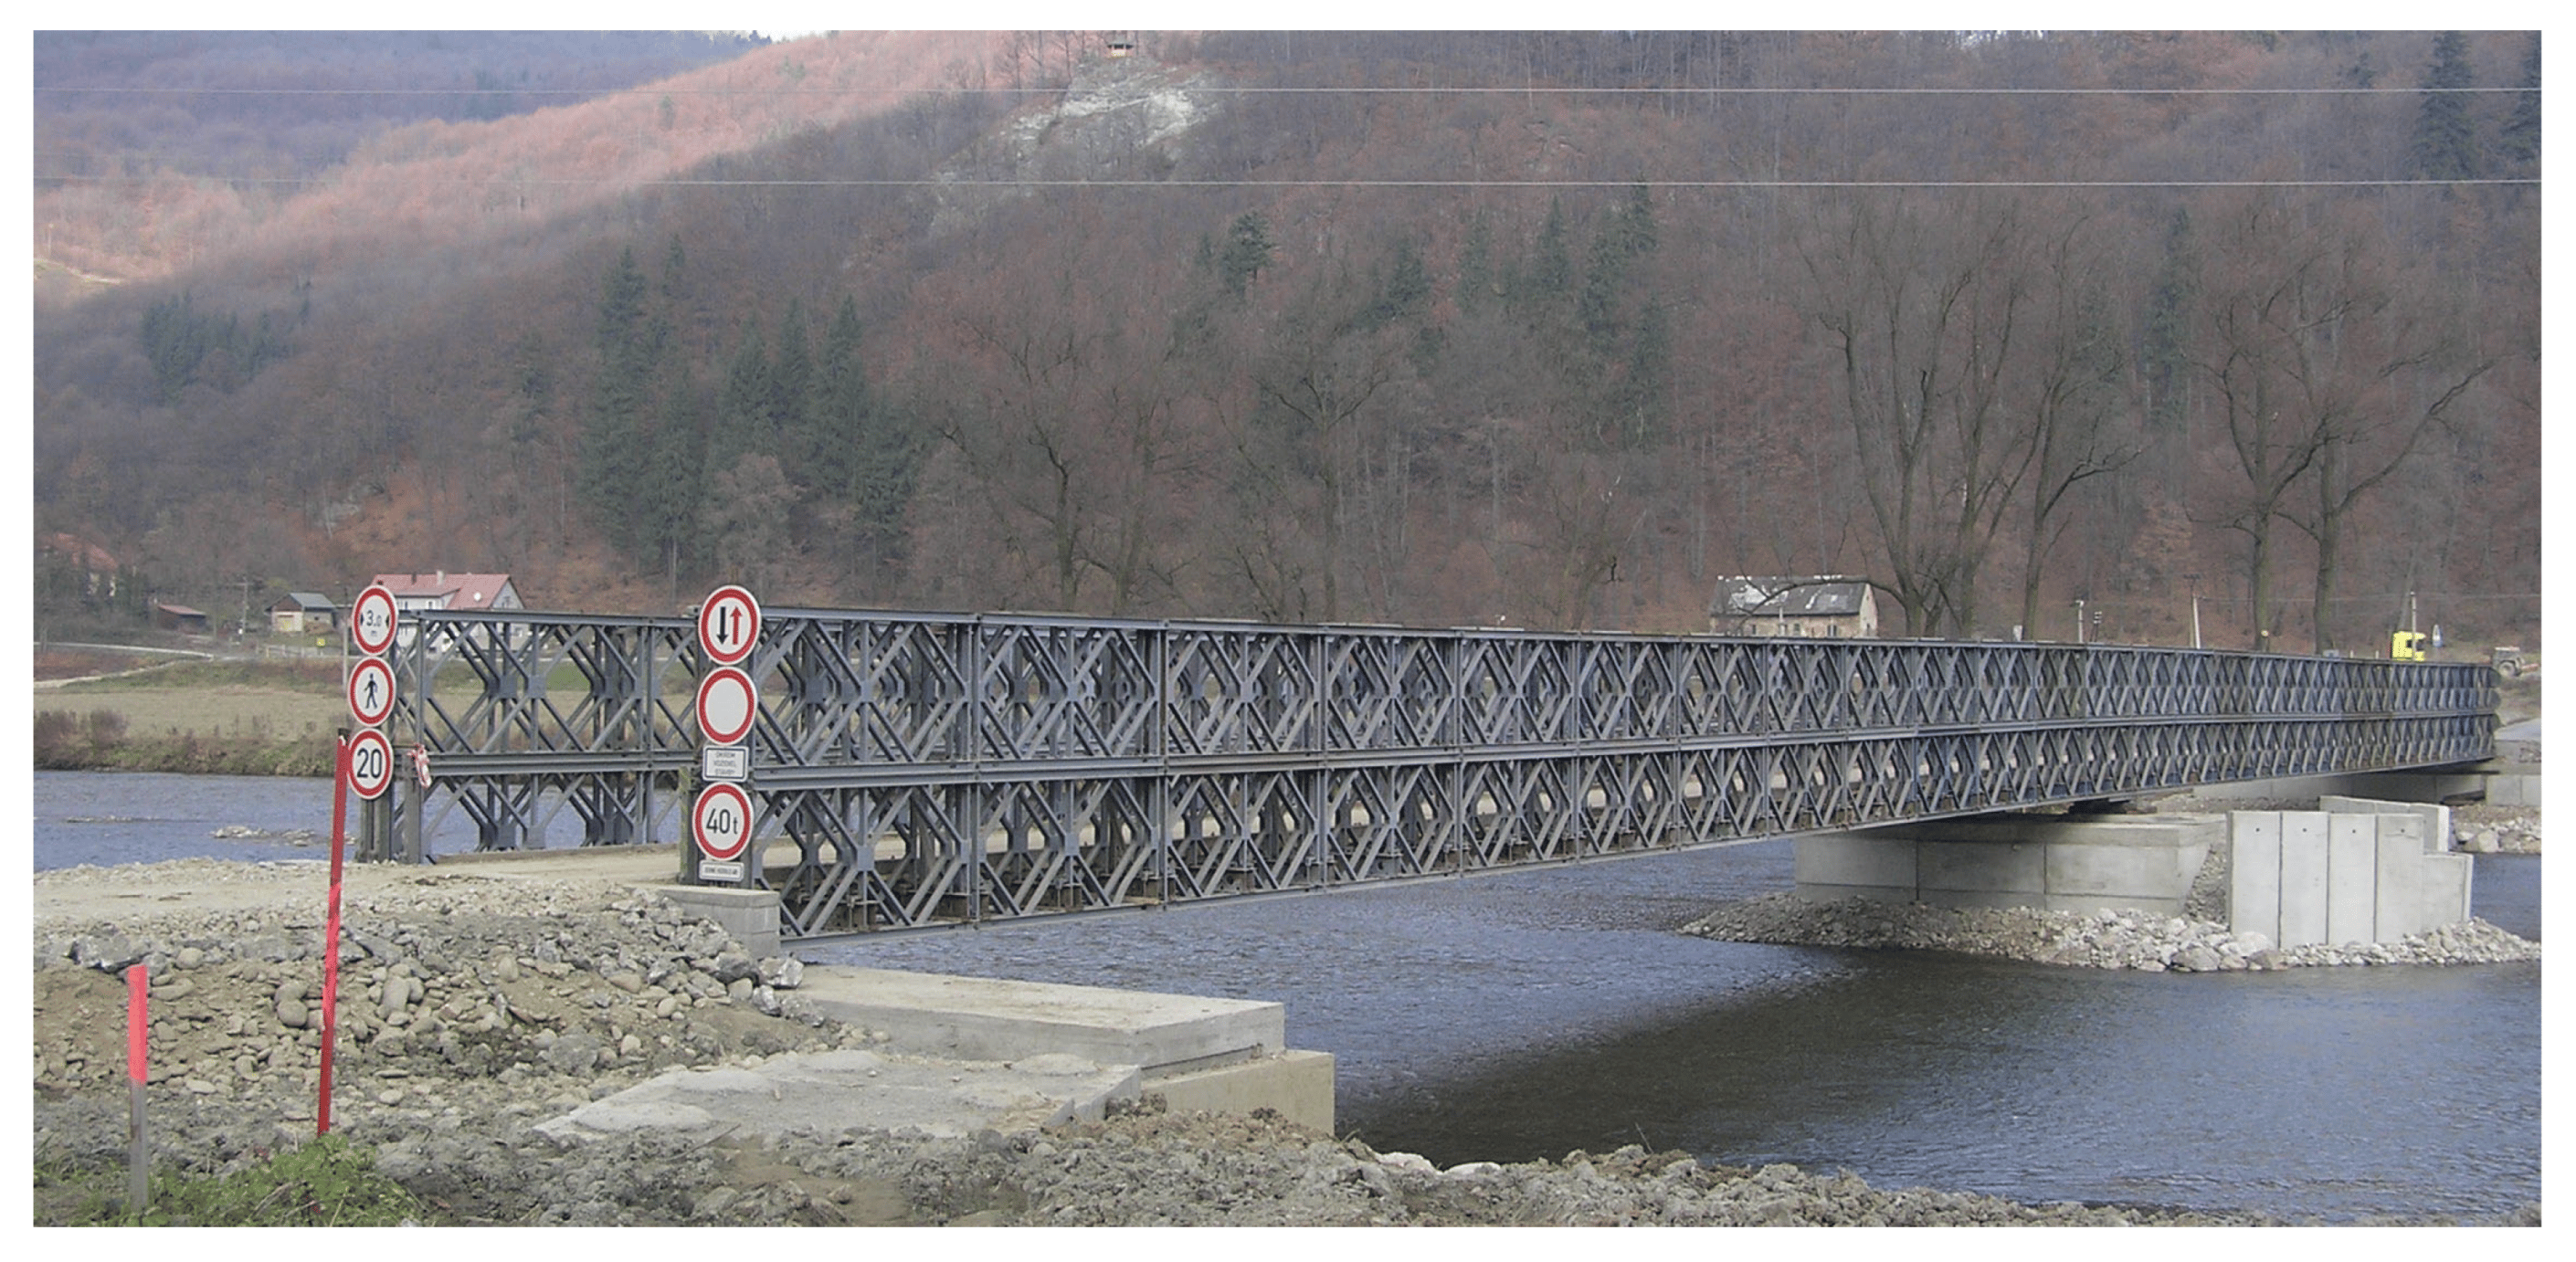
\includegraphics[width=\linewidth]{figures/06_DMO/00_bailey_bridge/applsci-12-03788-g002.png}
    \caption{Bailey bridge placed on construction site road over Orava river (Slovakia) \cite{prokop_load-carrying_2022}. }
    \label{fig:06_bailey}
\end{marginfigure}

The considered structure is a large modular structure based on the design of the Bailey bridge \sidecite{department_of_the_army_bailey_1986}. This concept has initially been studied for military purposes and later applied in civil engineering, particularly in temporary bridge structures. Its adaptability, low weight, and rapid erection, allowing almost immediate usability for traffic, make it highly versatile (see \figref{fig:06_bailey}). The structure consists of 20 modules in length and 2 modules in height. Each module measures \qty{3.050}{m} in length (\qty{10}{ft}) and \qty{1.525}{m} in height (\qty{5}{ft}). This configuration results in a total bridge span of \qty{30.50}{m} (\qty{100}{ft}).

The test case is based on the specifications given by Tugilimana \etal \sidecite{tugilimana_spatial_2017, tugilimana_integrated_2019} and is illustrated in \figref{fig:06_tug_bcs}, along with the geometrical and material data (normalized) utilized for the optimization (\tabref{tab:06_modular_tug}). The optimization is conducted only on the symmetric part of the structure. All constraints from the formulation \eqrefnotext{eq:06_optim_complete} are considered in this load case, excluding the buckling constraint, following the approach adopted by Tugilimana.


\begin{figure}
    \centering
    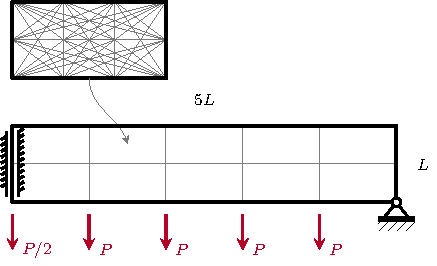
\includegraphics{figures/06_DMO/00_tug_bench_bcs/bcs.pdf}
    \caption{Graphical representation of the 2D Bailey bridge test case. The structure is divided into $N_\text{sub}=10$. The bridge is symmetric, and we are here optimizing only the right part of it.}
    \label{fig:06_tug_bcs}
\end{figure}

\begin{margintable}
    \small
    \centering
    \begin{tabular}{cc}
    \toprule
    \textbf{Parameter}        & \textbf{Value} \\ \midrule
    $L$              & 3.05     \\
    $\sigma_\text{c}, \sigma_\text{t}$ & $\pm 1$\\
    $P$              & 1   \\
    \bottomrule
    \end{tabular}
    \caption{Material data used for the 2D Bailey bridge without local buckling constraints test case to compare with the work of Tugilimana \etal \cite{tugilimana_integrated_2019}.}
    \label{tab:06_modular_tug}
\end{margintable}

The resulting optimized structures are presented in the right part of \figref{fig:00_tug_bench}, alongside the topology of the structures optimized by Tugilimana \etal \cite{tugilimana_integrated_2019}. Below each subfigure, the structure volume is provided, along with the value relative to the Tugilimana solution in square brackets. While the reference images (left part of the image) do not highlight the submodules with the same module topology, it can be observed that the module layout is not always the same, as seen in the cases of $N_\text{T}=4$ or $N_\text{T}=5$. It is noteworthy that the proposed optimization algorithm not only excels in optimizing an intrinsically discrete optimization problem using continuous design variables and a gradient-based optimizer but also improves upon the results found in the literature by up to \qty{3}{\percent}. The structure obtained with $N_\text{T}=10$ is exactly the same as what would be achieved by optimizing the structure without considering the modular constraints.

\begin{figure*}
    \centering
    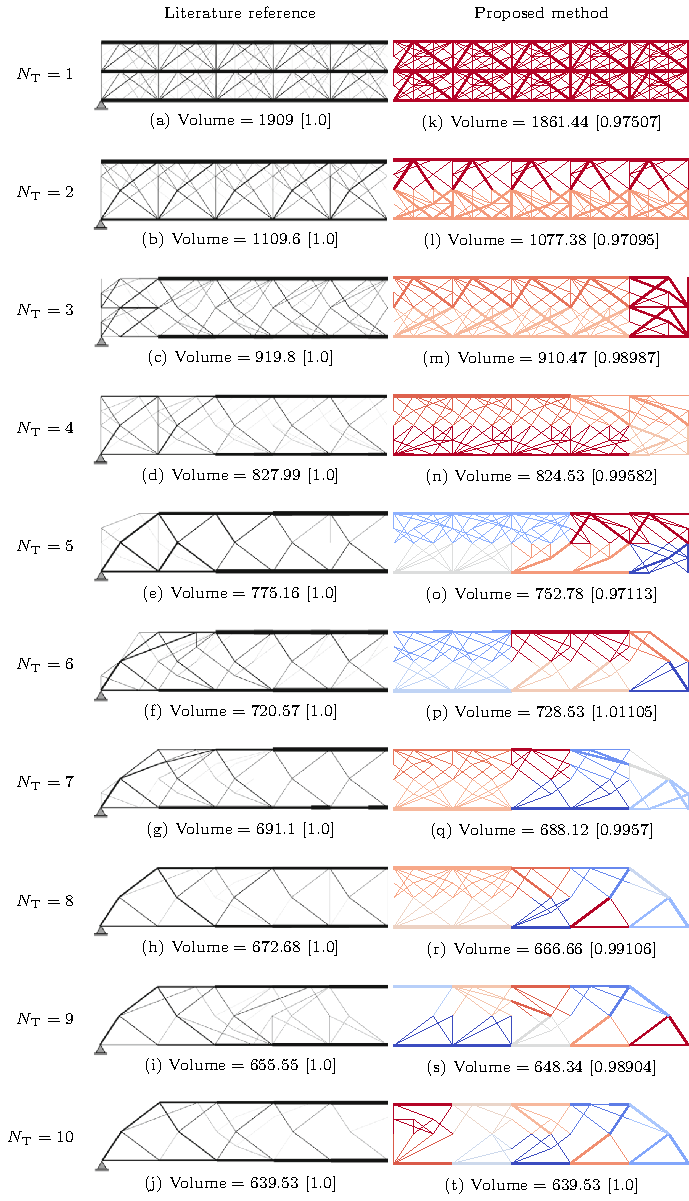
\includegraphics{figures/06_DMO/00_tug_bench/bench.pdf}
    \caption{Visual comparison of the 2D Bailey bridge test case without local buckling constraints proposed by Tugilimana \etal \cite{tugilimana_integrated_2019} obtained for different number of modules $N_\text{T}$. The images (a-j) represent the Tugilimana optimized structures, while the images (k-t) show the structures obtained with the proposed optimization method.}
    \label{fig:00_tug_bench}
\end{figure*}

Up until now, we always used normalized material data and dimensions, and we never considered local buckling of the truss. For this reason, we are interested in testing what happens in this specific test case when we do consider local buckling and use a real load case with realistic dimensions and material data. We are particularly interested in seeing if these changes significantly affect the module's topology and layout in the structure. The material data used for the optimization is presented in \tabref{tab:06_modular_tug_buck} and represents a generic aluminum. The cross-sections are assumed to be circular for the local buckling evaluation. Topological buckling is taken into account inside the modules, as explained in \secref{sec:05_topological}.

\begin{margintable}
    \small
    \centering
    \begin{tabular}{cc}
    \toprule
    \textbf{Parameter}        & \textbf{Value} \\ \midrule
    $L$              & \qty{3.05}{m}     \\
    $E$              & \qty{69}{GPa}     \\
    $\sigma_\text{c}, \sigma_\text{t}$ & $\pm $\qty{270}{MPa} \\
    $P$              & \qty{1}{MN}   \\
    \bottomrule
    \end{tabular}
    \caption{Material data used for the 2D Bailey bridge with local buckling constraints test case.}
    \label{tab:06_modular_tug_buck}
\end{margintable}

The optimized structures for the Bailey bridge with buckling constraints are shown for different numbers of module topologies ($N_\text{T}=1$ to 10) in \figref{fig:06_tug_bench_buck}. Quickly comparing them with the results without buckling, we notice that for this test case, the layout of the modules remains unchanged. The topology, however, is very different, with generally slightly fewer active bars. The volume can not be directly compared, so we normalize them with respect to the maximum volume ($N_\text{T}=1$) and plot them in \figref{fig:06_cant_volume_norm}. We notice that adding multiple module topologies is beneficial in the same exact way with or without buckling constraints. We can also comment that the biggest reduction in volume from the inclusion of additional modules comes especially at the beginning, e.g., going from $N_\text{T}=1$ to $N_\text{T}=2$ or from $N_\text{T}=2$ to $N_\text{T}=3$, while the difference at higher numbers is marginal as the succession approaches a plateau.

\begin{marginfigure}
    \centering
    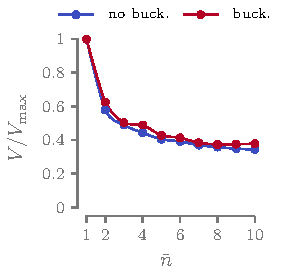
\includegraphics{figures/06_DMO/00_tug_bench_crv/vol.pdf}
    \caption{Normalized volume values plotted against the number of modules $N_\text{T}$. The buckling constraints do not change the trend of the beneficial effect of using multiple modules $N_\text{T}$ on the structure.}
    \label{fig:06_cant_volume_norm}
\end{marginfigure}

\begin{figure}
    \centering
    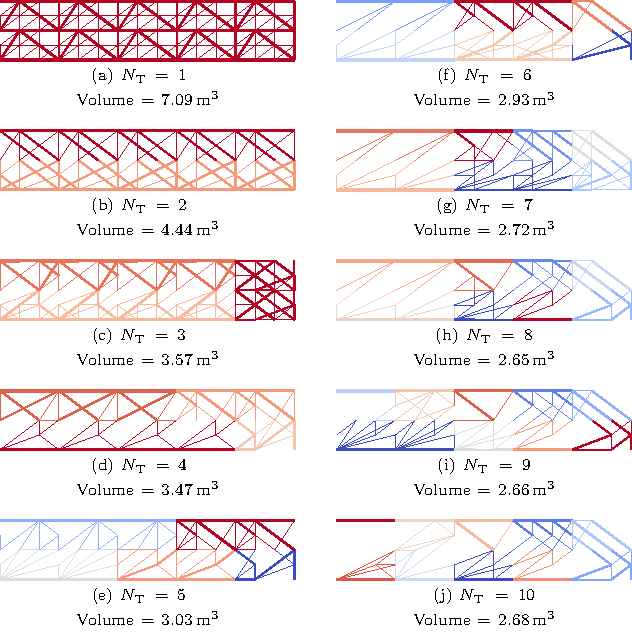
\includegraphics{figures/06_DMO/00_tug_bench_buck/buck.pdf}
    \caption{Visual representation of the optimized structures obtained for different values of $N_\text{T}$ for the 2D Bailey bridge test case with local buckling constraints.}
    \label{fig:06_tug_bench_buck}
\end{figure}

Willing to explore how different parameters can influence the resulting volume, topology, and layout, we optimize the same test case with a different number of subdomains and modules. We use the same test case, with the only difference being that we are now using a 3x2 nodes fully connected ground structure for faster calculation times.

\begin{figure*}
    \centering
    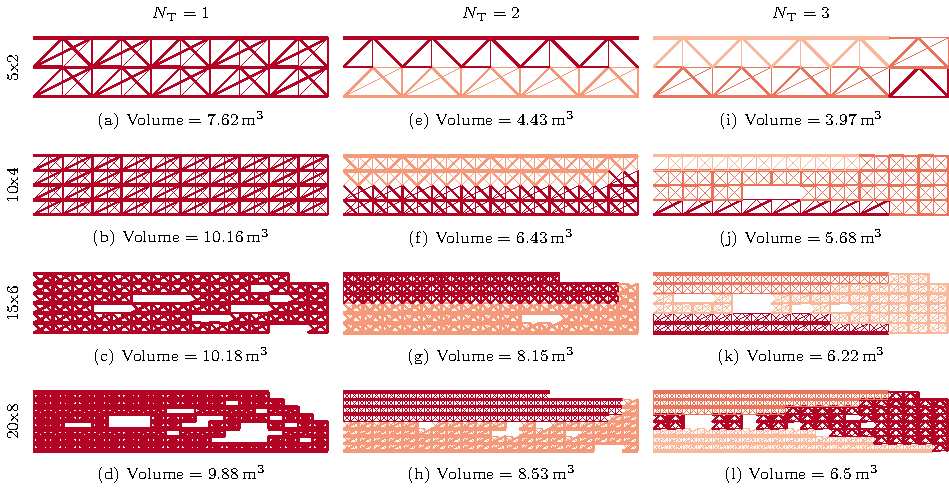
\includegraphics{figures/06_DMO/00_tug_bench_size/size.pdf}
    \caption{Study of the influence of the parameters $N_\text{sub}$ and $N_\text{T}$ on the volume and the topology of the 2D Bailey bridge test case.}
    \label{fig:06_size_res}
\end{figure*}

The results of the optimizations with different numbers of subdomains and modules are shown, together with the value of the structural volume in \figref{fig:06_size_res}. Looking at the the image from left to right, we observe that the trend of volume reduction with the increase in the number of module topologies we have already acknowledged previously is still valid. It is, however, more interesting to see what happens going from top to bottom, \ie what happens when we change the number of subdomains $N_\text{sub}$ without changing the number of module topologies $N_\text{T}$. As expected and already observed using the variable linking algorithm (see, for example, \figref{fig:05_scale_v} in Chapter~\ref{chap:05}), the volumes increase with the number of subdomains. However, in \figref{fig:06_cant_volume_norm_2}, in this case, we observe a steep increase in the structural volume and then a plateau, different from before. We speculate that this beneficial behavior comes mainly for two reasons: first, the optimization algorithm allows subdomains to show a completely empty topology. We observe that when we have not many subdomains, the structure is always fully filled, with no empty subdomains. But with the increasing number of subdomains, we notice more and more empty subdomains, helping to keep the structure light. Second, by increasing the number of subdomains, the average length of the subdomains' bars decreases. This phenomenon allows the change in the failure mode, moving from buckling to stress. For example, we observe that in \figref{fig:06_size_res}d, where the failure mode is completely changed to stress, and the module presents a symmetric topology, with equal stress distribution in compression and tension. This is a very effective use of the material, and consequently, the volume decreases.


\begin{marginfigure}
    \centering
    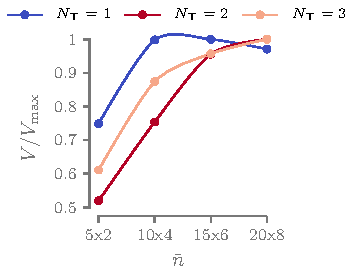
\includegraphics{figures/06_DMO/00_tug_bench_crv2/vol.pdf}
    \caption{Normalized volume values plotted against the number of subdomains $N_\text{sub}$ for different values of $N_\text{T}$.}
    \label{fig:06_cant_volume_norm_2}
\end{marginfigure}

Lastly, we observe that the modules' layout is almost invariant with the increasing number of subdomains. This fact is somewhat similar to what we observe in classic topology optimization when we increase the mesh fineness with a distance-based filter. In these cases the topology remains unchanged with mesh refinement.

\subsection{Simply supported 3D beam}
The last test we conduct is on the simply supported 3D beam, a load case introduced in Chapter~\ref{chap:04} and already used throughout this thesis. We recall the test case and the material and geometric data used for the optimization process in \figref{fig:06_symm_support_bc} and \tabref{tab:06_3D_supp_mat}. As already done, we optimize here only one-fourth of the entire structure thanks to its symmetry planes. We conduct the optimization using 6x2x3 subdomains on the X, Y, and Z axes, respectively, and every module is discretized using a 3x3x3 fully connected ground structure with a total number of candidates $\bar{n} = 351$ per module. The optimization is conducted using three different numbers of modules, $N_\text{T}=1$, 2, 3.

\begin{marginfigure}
    \centering
    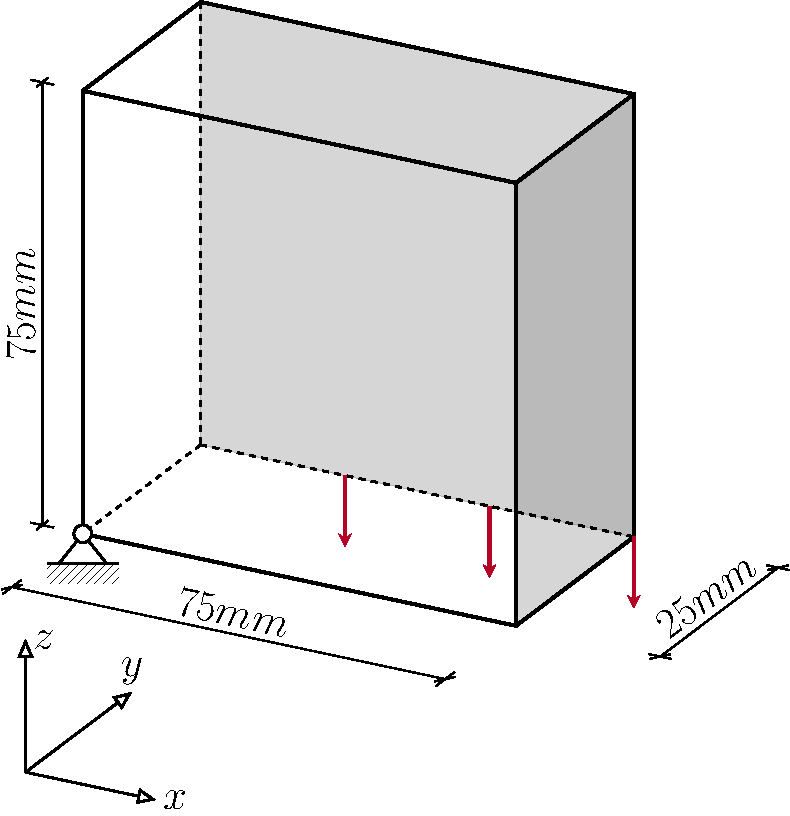
\includegraphics[width=\linewidth]{figures/06_DMO/00_supported_bc/supported_3D_symm.pdf}
    \caption{Symmetric boundary conditions of the simply supported 3D beam. In gray are the symmetry planes of the test case.}
    \label{fig:06_symm_support_bc} 
\end{marginfigure}

\begin{margintable}
    \small
    \centering
    \begin{tabular}{cc}
    \toprule
    \textbf{Parameter}        & \textbf{Value} \\ \midrule
    $E$              & \qty{2.7}{GPa}     \\
    $\sigma_\text{c}, \sigma_\text{t}$ & $\pm $\qty{55}{MPa} \\
    $\rho$              & \qty{1.14}{\gram\per\cubic\centi\metre}   \\
    $P$              & \qty{100}{N}   \\
    \bottomrule
    \end{tabular}
    \caption{Material data used for the simply supported 3D beam optimization.}
    \label{tab:06_3D_supp_mat}
\end{margintable}

The resulting optimized structures are presented in \figref{fig:06_supp_top}, and the associated numerical results are presented in \tabref{tab:06_supp_tab}. The first observation is that in this specific test case, the optimizer converges to solutions in which the sum of alpha for every subdomain is equal to one. While previously, we have seen that the formulation arrived at creating empty subdomains where the sum of alpha is zero (see \figref{fig:06_diferent_modules_cant_topology} or \figref{fig:06_size_res}), here the optimizer failed in doing so. The empty subdomains for $N_\text{T}=2$ and $N_\text{T}=3$ correspond to cases where the cross-sectional areas of one module are set to zero, and the optimizer puts the value of the corresponding alpha to one. In this way, the solution is still optimized correctly, but using one module topology en plus. For example, looking at \figref{fig:06_supp_top}b and e, the solution for $N_\text{T}=2$ shows that the optimized structure exhibits only one module topology, the other being empty.

We speculate that this problem arises from the optimizer's settings used to normalize the design variables and constraints for the optimization. For instance, even after scaling the layout design variable $\vect{\alpha}$ and its corresponding constraints with multiple values, we consistently obtained the same results. This issue suggests that while the starting point perturbation certainly aids in achieving a well-optimized structure, additional work is needed to develop a new resolution strategy. One possible approach could be to separate the topology and layout variables and iteratively solve the two problems independently, one iteration at a time.

Despite encountering this issue, a careful examination of the volume $V$ and mean densities $\bar{\rho}$ in \tabref{tab:06_supp_tab} reveals that the modular structures with $N_\text{T}=2$ and $N_\text{T}=3$ achieve remarkably similar values to the monolithic reference ($N_\text{sub}=1$) depicted in \figref{fig:06_supp_ref}. This outcome is particularly significant as it attains the objective of achieving a lightweight structure, almost comparable to the monolithic one, while preserving modularity, highlighting the potential for a lighter structure with manufacturing advantages due to its modular nature.

\begin{figure*}
    \hspace*{\fill}
    \subcaptionbox{}{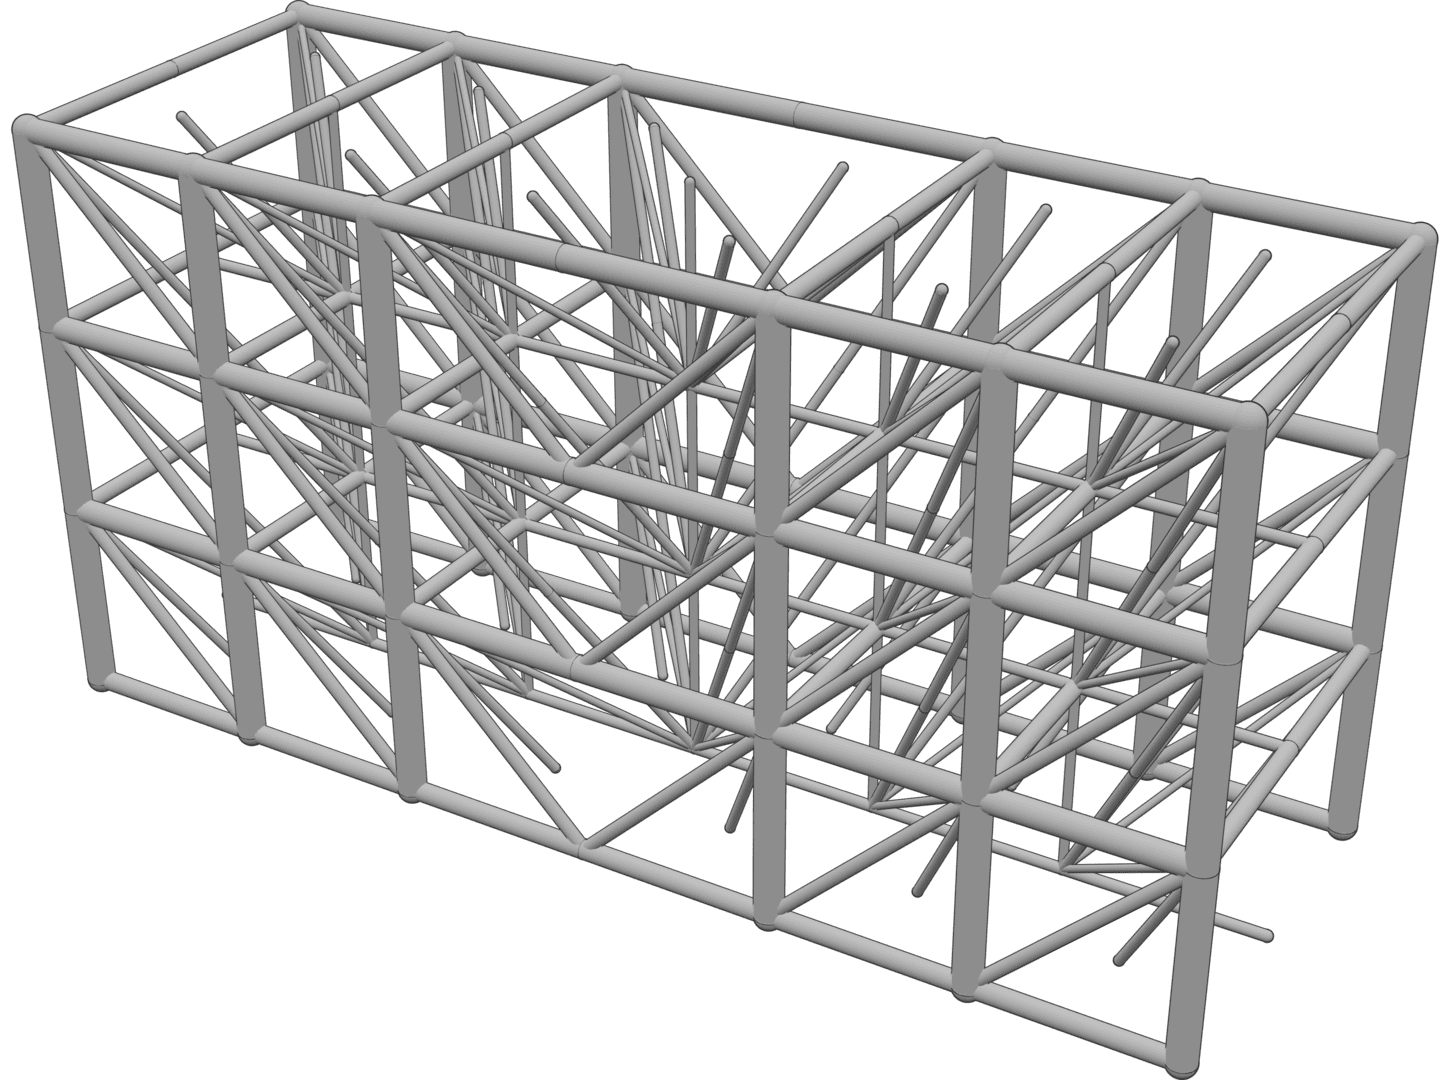
\includegraphics[width=0.30\linewidth]{figures/06_DMO/00_print_topology/1_04_Topology_NLP_iso.png}}
    \hfill
    \subcaptionbox{}{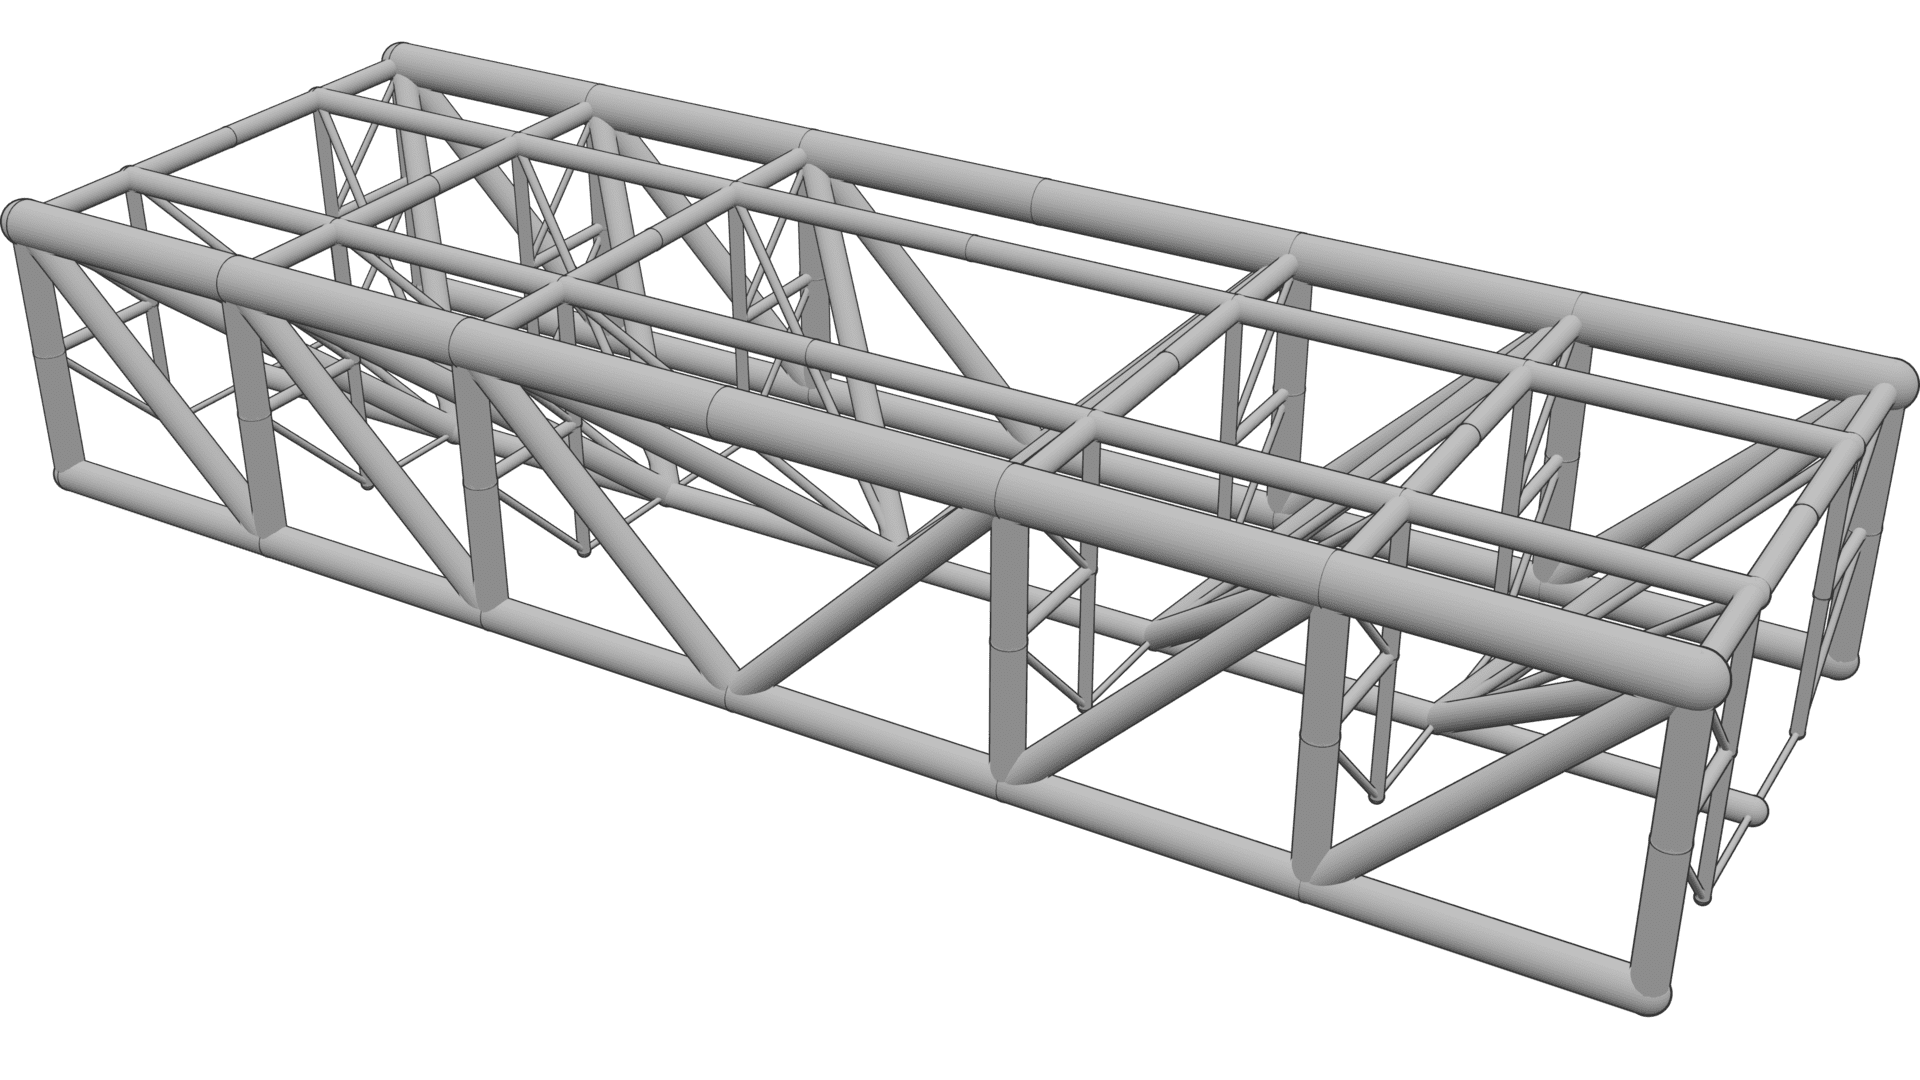
\includegraphics[width=0.30\linewidth]{figures/06_DMO/00_print_topology/2_04_Topology_NLP_iso.png}}
    \hfill
    \subcaptionbox{}{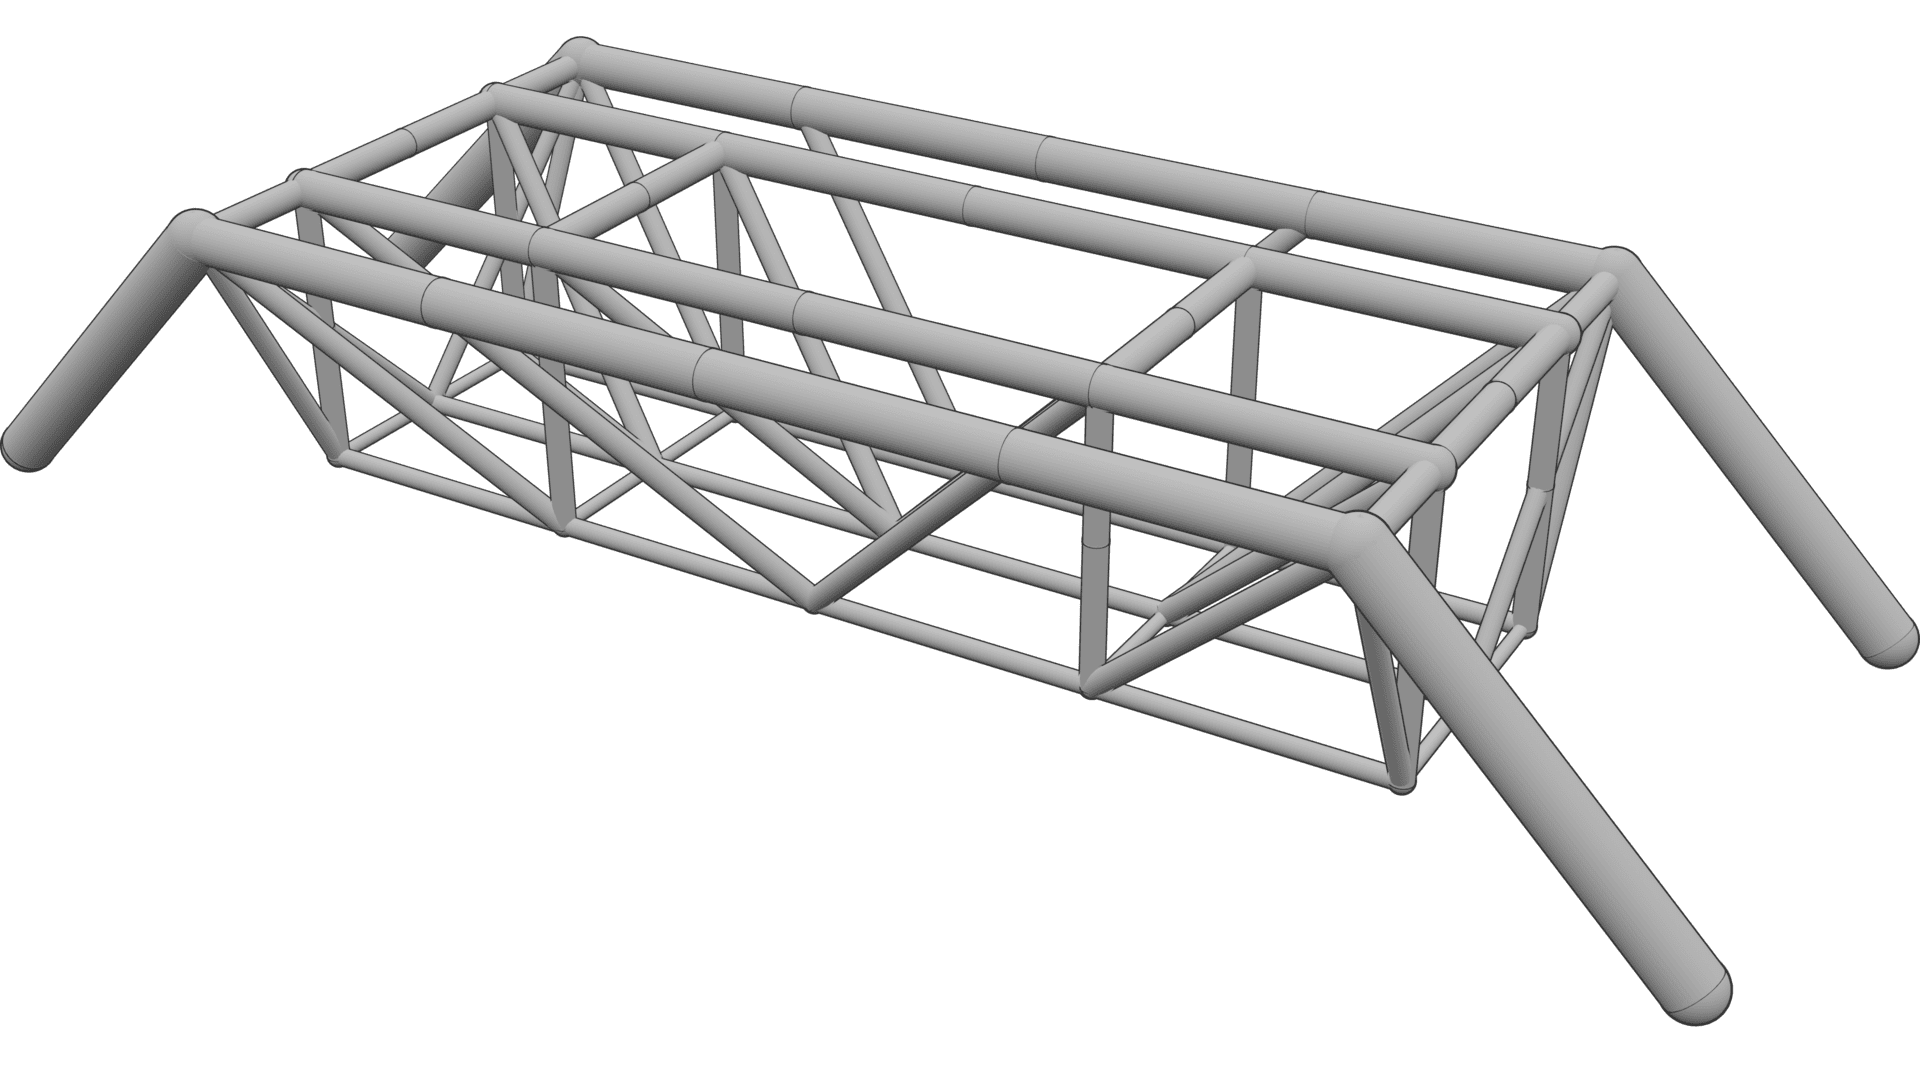
\includegraphics[width=0.30\linewidth]{figures/06_DMO/00_print_topology/3_04_Topology_NLP_iso.png}}
    \hspace*{\fill}
    \bigskip
    \hspace*{\fill}
    \subcaptionbox{}{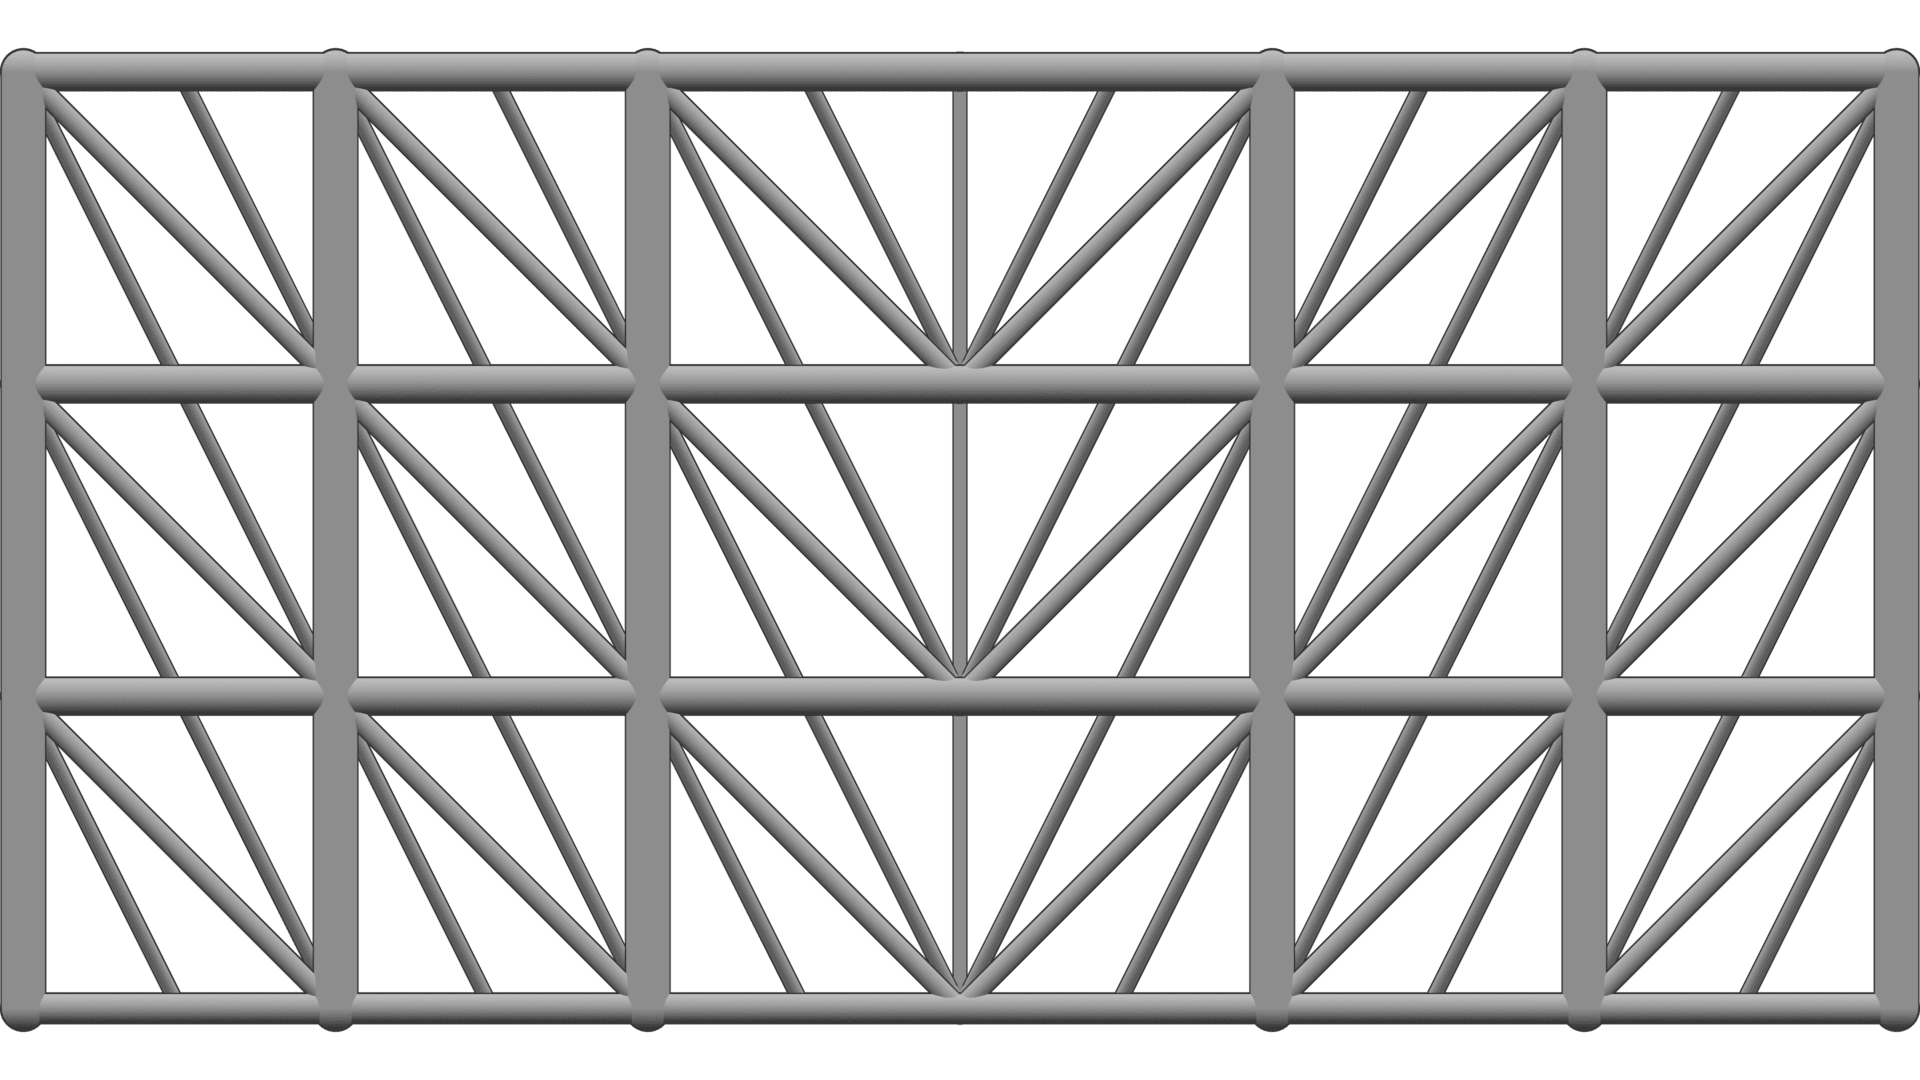
\includegraphics[width=0.30\linewidth]{figures/06_DMO/00_print_topology/1_04_Topology_NLP_XZ.png}}
    \hfill
    \subcaptionbox{}{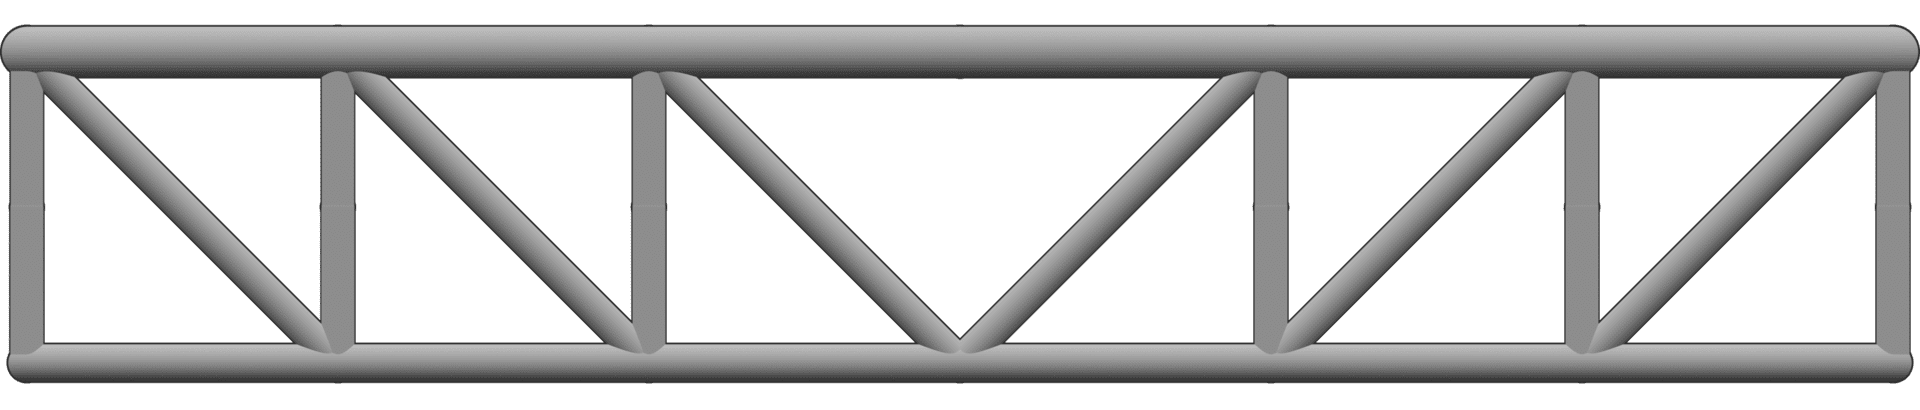
\includegraphics[width=0.30\linewidth]{figures/06_DMO/00_print_topology/2_04_Topology_NLP_XZ.png}}
    \hfill
    \subcaptionbox{}{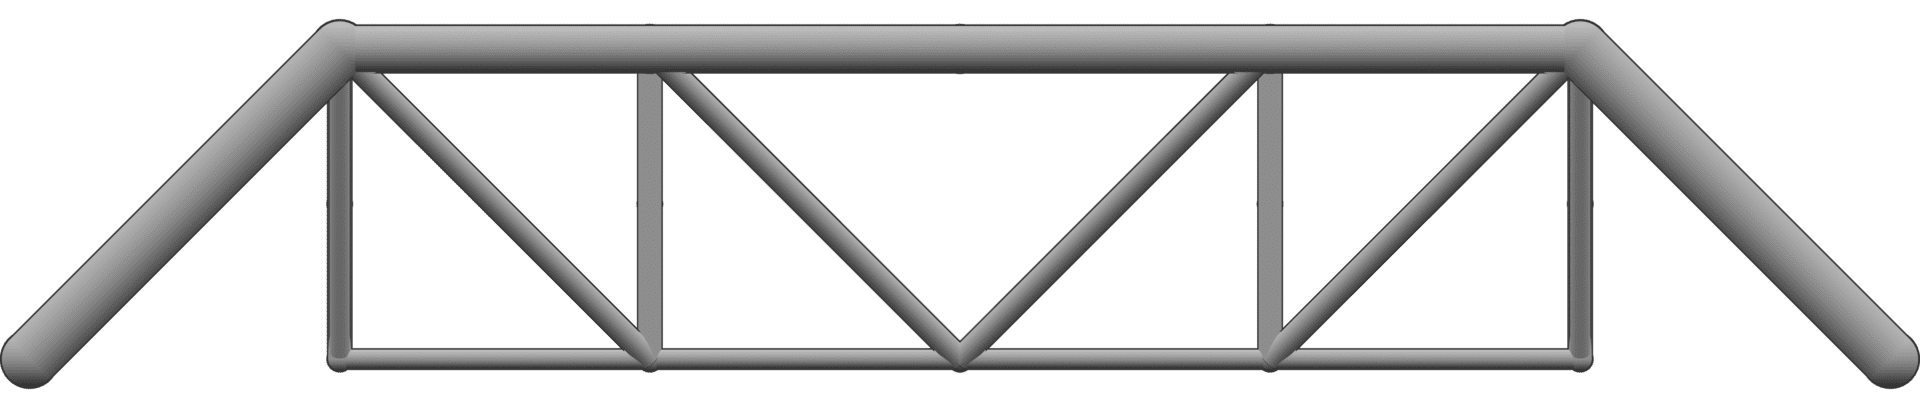
\includegraphics[width=0.30\linewidth]{figures/06_DMO/00_print_topology/3_04_Topology_NLP_XZ.png}}
    \hspace*{\fill}
    \caption{Rendering of the optimized structures with $N_\text{T}=1$ (a,d), $N_\text{T}=2$ (b,e), and $N_\text{T}=3$ (c,f).}
    \label{fig:06_supp_top}
\end{figure*}

\begin{table}
    \centering
    \small
    \begin{tabular}{lx{1.8cm}x{1.8cm}x{1.8cm}x{1.8cm}}
        \toprule
    $N_\text{T}$ & --     & 1     &  2    &  3  \\ \midrule
    $N_\text{sub}$           &    1  &   36   &   36   &   36     \\
    $N_\text{opt}\;(N_\text{el})$  &  20 (1984) &  360 (12636)   &  204 (12636)   &  104 (12636)        \\
    $V$ [\unit{cm^3}] & 9.907 &  27.958 &   15.548  & 10.178    \\
    $V$ [\unit{\percent}] & 1.761 & 4.970&2.764 & 1.809    \\
    $\bar{\rho}$ [\unit{kg/m^3}] & 80.31 &226.65 &126.05 &82.51 \\
    % C [\unit{J}]      &  3.71  &  5.20   &  6.21  & 4.14  \\
    % $a_\text{max}$ [\unit{mm^2}]      & 37.61& 9.40  & 12.81  &   15.81     \\
    $\varphi$   &\qty{100.00}{\percent}&\qty{21.11}{\percent}&\qty{39.21}{\percent}&\qty{80.77}{\percent}  \\
    $\psi$& 1.00   &  0.47 &  0.66   & 0.87        \\
    t        & \hms{0;0;4}  &  \hms{0;1;18} & \hms{0;0;42} & \hms{0;10;22}   \\ \bottomrule
    \end{tabular}
    \caption{Numeric results of the parametric study on the influence of the number of modules $N_\text{T}$ on the simply supported 3D beam.}
    \label{tab:06_supp_tab}
    \end{table}

    \begin{marginfigure}
        \centering
        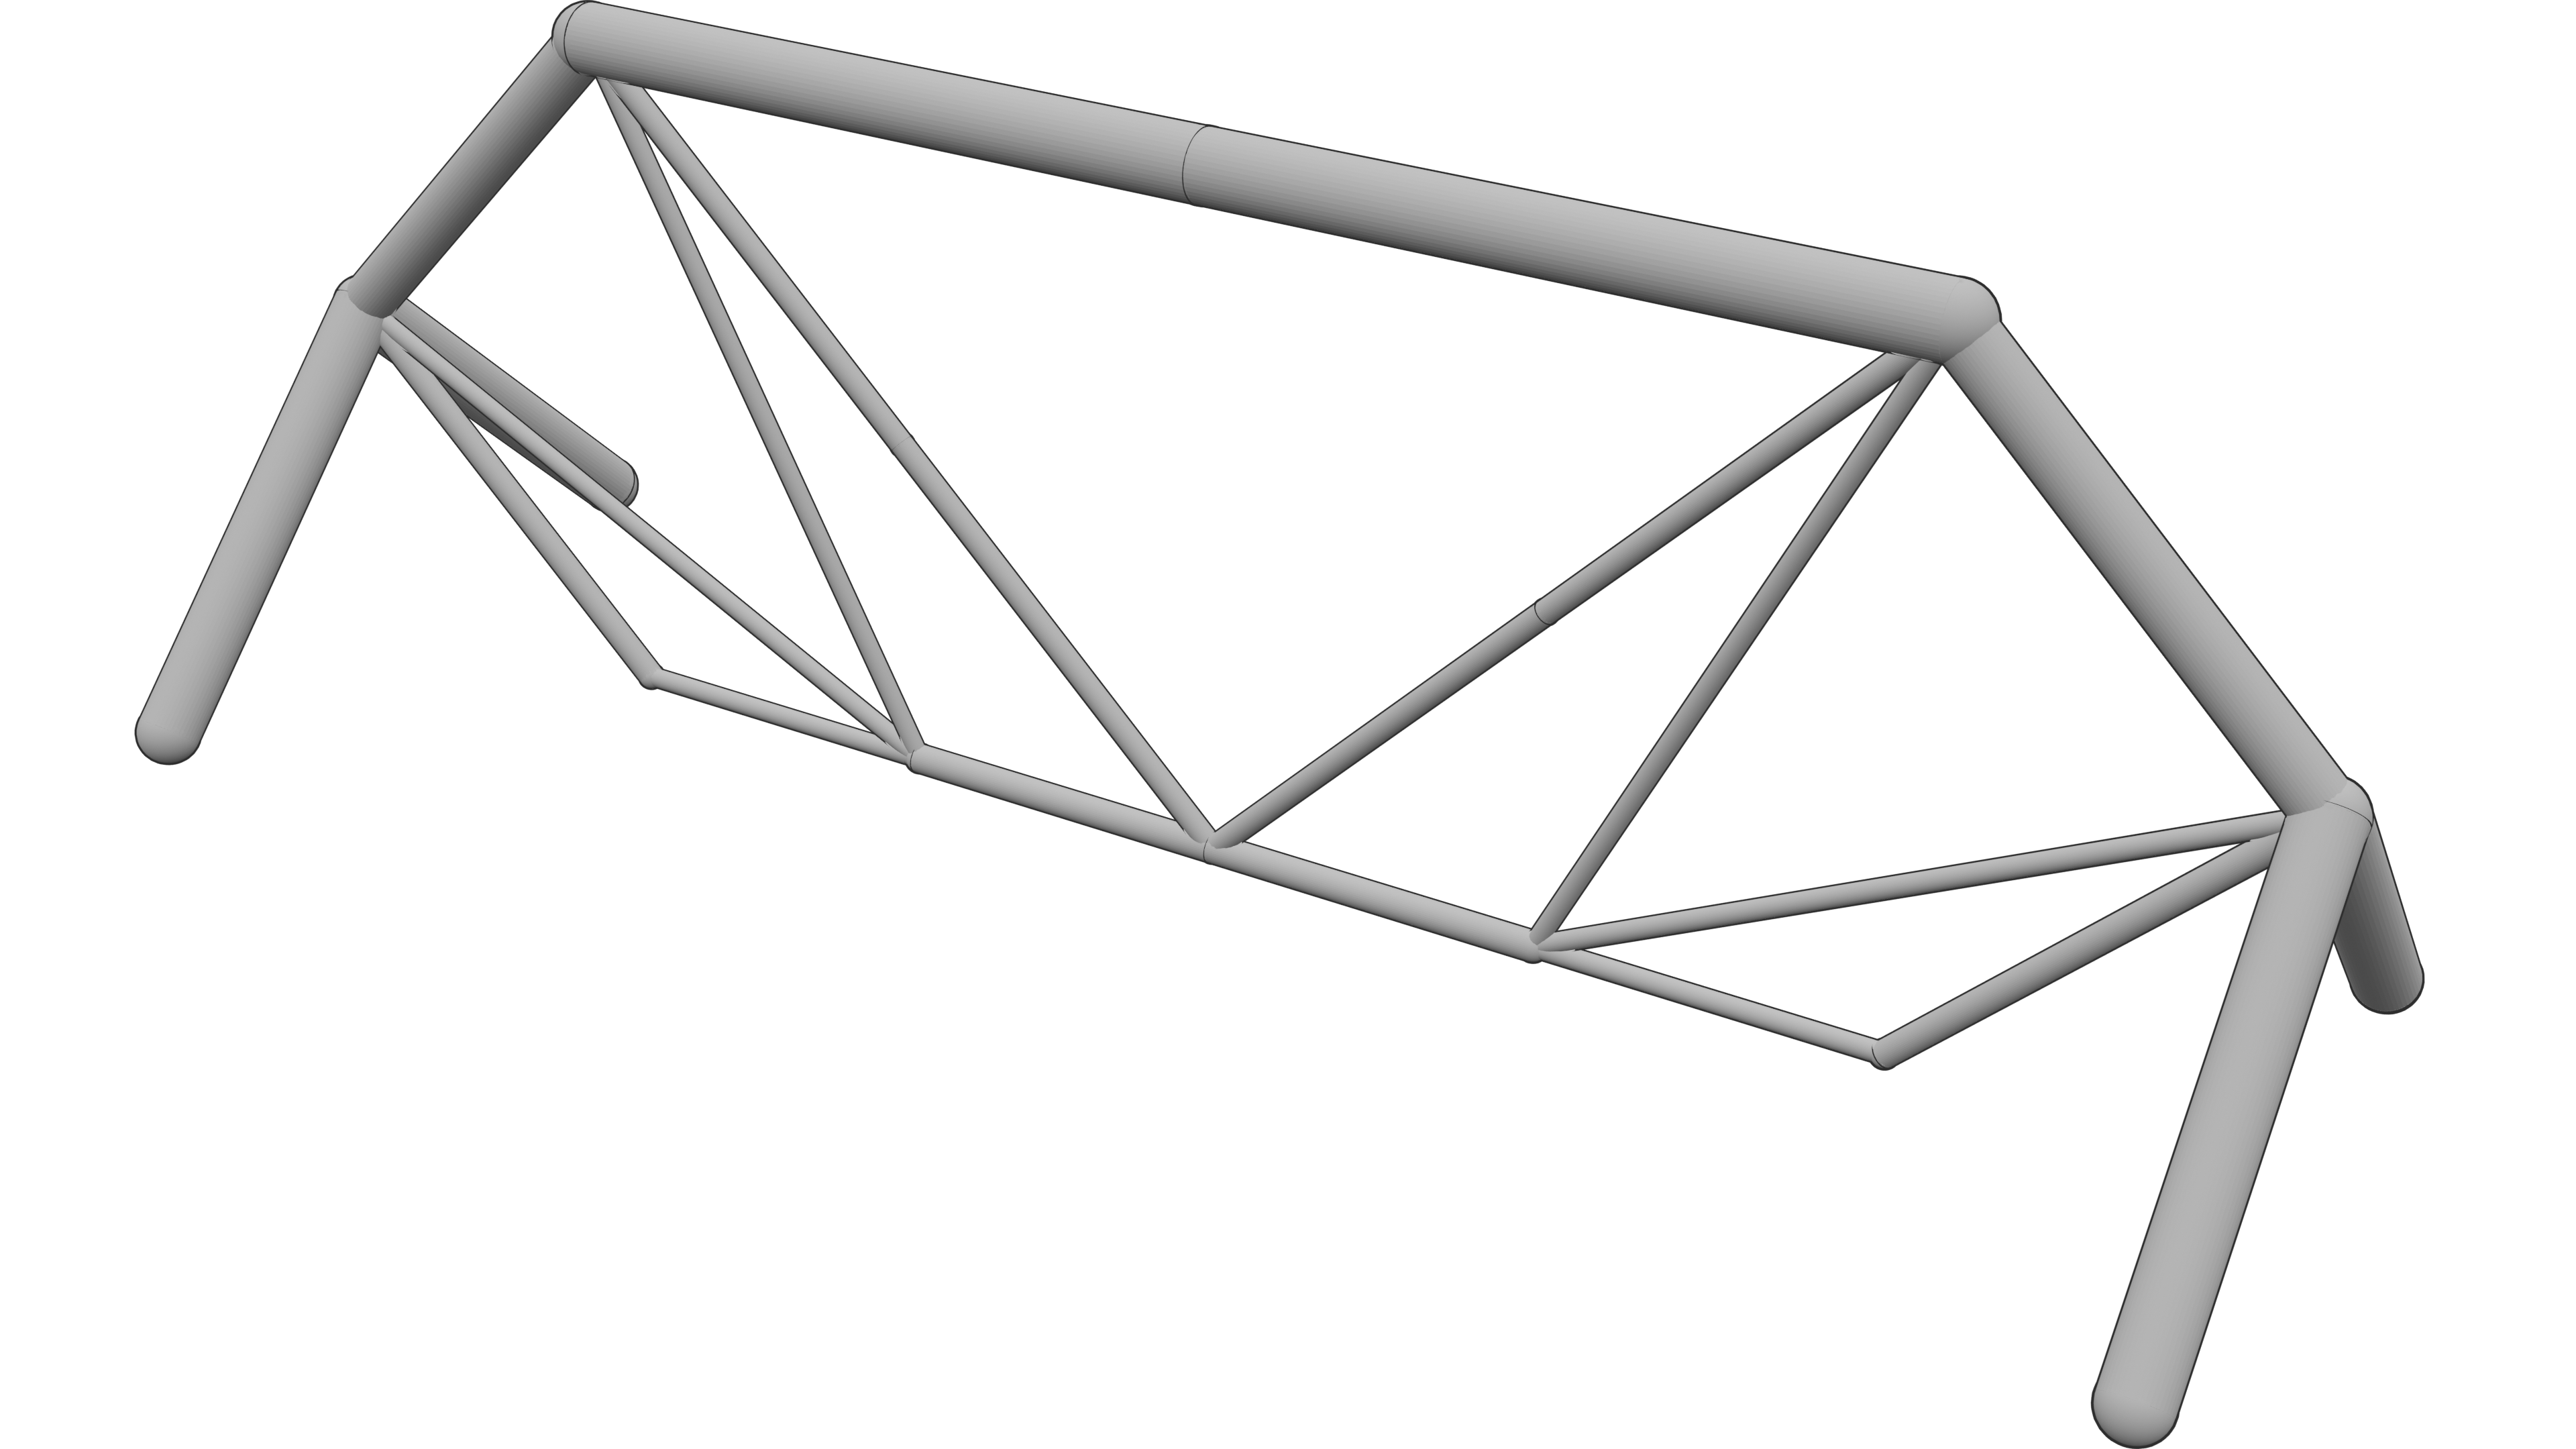
\includegraphics[width=\linewidth]{figures/04_TTO_improvements/16_supported_3D_sol/04_Topology_NLP_iso-min.png}
        \caption{Perspective view of the monolithic simply supported 3D beam optimized structure with $V=\qty{9.907}{\centi\meter^3}$.}
        \label{fig:06_supp_ref}
    \end{marginfigure}

\section{Conclusion}
In this chapter, we introduced an innovative optimization formulation designed to optimize the structural volume of modular structures. The solving algorithm leverages the physical information of the model, exploiting analytical derivatives and employing a gradient descent optimization approach. Categorical variables, used to determine module layout, are modeled using a weighted sum of continuous weights that align with the continuous design variables of the optimization scheme. A double penalization scheme is proposed to mitigate the occurrence of non-physical intermediate weights.

The proposed formulation is tested across a variety of two- and three-dimensional test cases sourced from the literature. These tests confirm that the utilization of this optimization formulation enables modular structures to achieve volumes very close to those obtained from monolithic optimization, maintaining modularity and offering a favorable tradeoff between optimality and manufacturing complexity. However, the focus has been on simple test cases lacking engineering relevance so far. In the next chapter, we address this limitation by applying the presented optimization formulations in the aerospace context.
